\documentclass{beamer}
\mode<presentation> {
	%\usetheme{Dresden}
	\usetheme{CambridgeUS}
}
\newcommand{\subitem}{\par\qquad}
\usepackage{booktabs}
\usepackage{mathtools}
\usepackage{amssymb}
\usepackage{amsthm}
\usepackage{tikz}
\usepackage{subfigure}	
\usepackage[round]{natbib}

\DeclareMathOperator*{\argmin}{argmin}
\DeclareMathOperator*{\argmax}{argmax}
\newtheorem{lem}{Lemma}
\newtheorem{thm}{Theorem}
\newtheorem{nots}{Note}
\newtheorem{defs}{Definition}



\newcommand{\independent}{\mbox{${}\perp\mkern-11mu\perp{}$}}
\newcommand{\notindependent}{\mbox{${}\not\!\perp\mkern-11mu\perp{}$}}
\newcommand{\iid}{\overset{\text{iid}}{\sim}}

\newcommand{\R}{\mathbb{R}}
\newcommand{\E}{\mathbb{E}}
%\newcommand{\C}{\mathbb{C}}

\newcommand{\y}{\mathbf{y}}
\newcommand{\uu}{\mathbf{u}}
\newcommand{\z}{\mathbf{z}}
\newcommand{\vv}{\mathbf{v}}
\newcommand{\w}{\mathbf{w}}
\newcommand{\x}{\mathbf{x}}

\newcommand{\Hyp}{\mathcal{H}}
\newcommand{\Myp}{\mathcal{M}}
\newcommand{\Ayp}{\mathcal{A}}

\newcommand{\Yspace}{\mathcal{Y}}
\newcommand{\Xspace}{\mathcal{X}}

\title[Online Learning]{Online Learning and Online Convex Optimization} 
\subtitle{Introduction and Some New Trends}

\author[Behrad Moniri - Mahdi Sabbaghi]{Behrad Moniri \and Mahdi Sabbaghi}


\institute[]{Department of Electrical Engineering\\Sharif University of Technology\\
	\vspace{2cm}
	Statistics Reading Group\\ Tehran Institute for Advanced Studies (TeIAS)
}

\date{}

%	\includegraphics[width=2cm]{digilogo.png}


\newcommand{\bigCI}{\mathrel{\text{\scalebox{1.07}{$\perp\mkern-10mu\perp$}}}}

\begin{document}
	\maketitle
	
	
	\frame{\tableofcontents}
	
	\section{Introduction}
	\frame{\sectionpage}
	\begin{frame}
	\frametitle{Introduction}
	\begin{itemize}
		
		
		
		
		\item Online learning is the process of answering a sequence of questions given (maybe partial) knowledge of the correct answers to previous questions and possibly additional available information.
		
		
		\pause
		\item  Many interesting theoretical properties and practical applications.
		
	\end{itemize}
\end{frame}


\begin{frame}
\frametitle{Setting}

\begin{figure}
	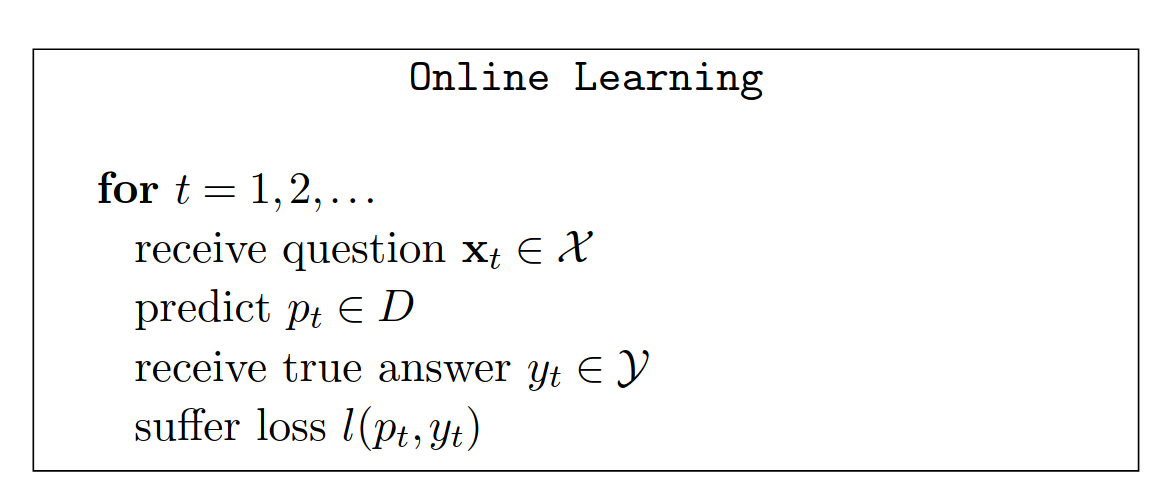
\includegraphics[scale=0.2]{./figures/setting.png}
\end{figure}

\begin{itemize}
	\item Online Classification
	\item Online Regression
	\item Learning from Expert Advice
	\item \textbf{Online Convex Optimization}
	
\end{itemize}

\end{frame}


\begin{frame}
\frametitle{Goals and Assumptions}

\begin{itemize}
\item The learner’s ultimate goal is to minimize the cumulative loss suffered along its run.
\pause
\item learning is hopeless if there is no relation between past and present rounds.
\pause
\item i.i.d. in classical statistical learning theory vs. adversarial in online learning.
\end{itemize}

\end{frame}

\begin{frame}
\begin{itemize}
\item Naturally, an adversary can make the cumulative loss to our online learning algorithm arbitrarily large.
\pause
\item It can ask the same question on each round, wait for the answer, and provide the opposite answer as the correct answer.
\pause
\item To make non-trivial statements, we make several natural assumptions.

\end{itemize}
\end{frame}

\begin{frame}
\frametitle{Two scenarios}
There are two main scenarios:

\begin{itemize}
\item \textbf{The Realizable Setting} (the simple one):

Answers are generated by some mapping $h^*: \Xspace \to \Yspace$ and $h^* \in \Hyp$.\\


\begin{itemize}
\item $\mathcal{H}$ is known by the learner.
\item $h^* \in \mathcal{H}$ is chosen by the adversary.
\end{itemize}
\pause

\item \textbf{Regret Setting} (the more interesting one): No longer assume answers are generated by $h^* \in \Hyp$, but require the learner to be competitive with the best fixed predictor from $\Hyp$:

\begin{equation}
\mathrm{Regret}_T(h^*) = \sum_{t = 1}^{T} l(p_t, y_t) - \sum_{t = 1}^{T} l(h^*(x_t), y_t)
\end{equation}

\begin{equation}
\mathrm{Regret}_T(\Hyp) = \max_{h^* \in \Hyp}  \; \mathrm{Regret}_T(h^*)
\end{equation}
Low regret algorithm: $o(T)$ Regret.

\end{itemize}
\end{frame}

\section{Realizable Setting}
\frame{\sectionpage}

\begin{frame}{Realizable Setting}
\begin{itemize}
\item Analogous to the PAC-Learning Setting
\item
With this restriction on the sequence, the learner should make as few mistakes as possible, i.e:
\begin{equation}
l_t(p_t, y_t)= \mathbf{1}\{p_t \neq y_t\}
\end{equation}

\pause

\item
Suppose we have given a sequence:
$$S= (x_1, h^*(y_1)), \hdots,  (x_T, h^*(y_T))$$
\textbf{Objective}: minimize $\mathcal{M}_{\mathcal{A}}(\mathcal{H}) := \underset{S \in \mathcal{S}}{\mathrm{sup}} \sum_{t=1}^N \mathbf{1}\{p_{A_t} \neq y_t\} $
\pause

\item
A bound on $\Myp_{\Ayp}(\Hyp)$ is called a \textbf{mistake-bound}
\end{itemize}

\end{frame}

\begin{frame}{Learnability}
\begin{defs}
We say that a hypothesis class $\Hyp$ is \textbf{online learnable} if there exists an algorithm $\Ayp$ for which $\Myp_{\Ayp}(\Hyp) < B < \infty$.
\end{defs}


\pause

\begin{itemize}
\item 
Let's start with a simplifying assumption: 
$|\Hyp|< \infty$

\pause

\item
basically, we can eliminate each $h$ with false output in every step. \pause \\ $\to$ Consistent Algorithm
\end{itemize}

\end{frame}

\begin{frame}{Consistent Algorithm}
\begin{figure}[h!]
\centering
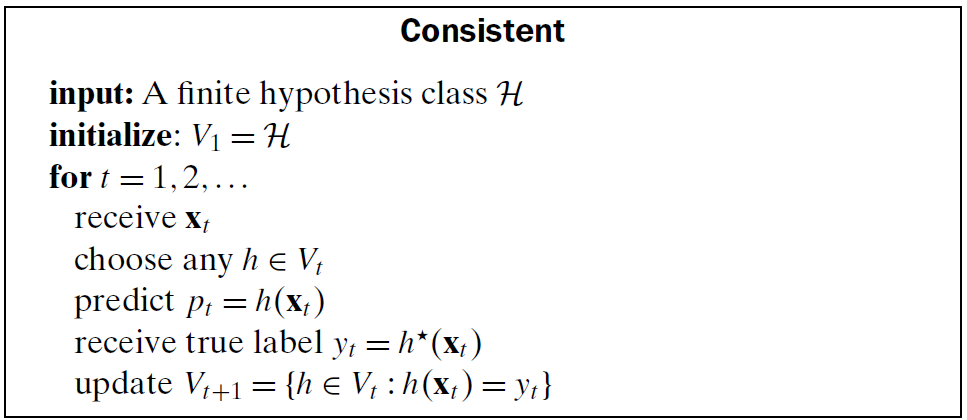
\includegraphics[width=0.8\textwidth]{./figures/Consistent.png}
\end{figure}

\pause
\begin{itemize}
\item 
It's easy to see that: 
\begin{equation}
\Myp_{\mathrm{Consistent}}(\Hyp) < |\Hyp|-1
\end{equation}
\end{itemize}
\end{frame}


\begin{frame}{Halving}
\begin{figure}[h!]
\centering
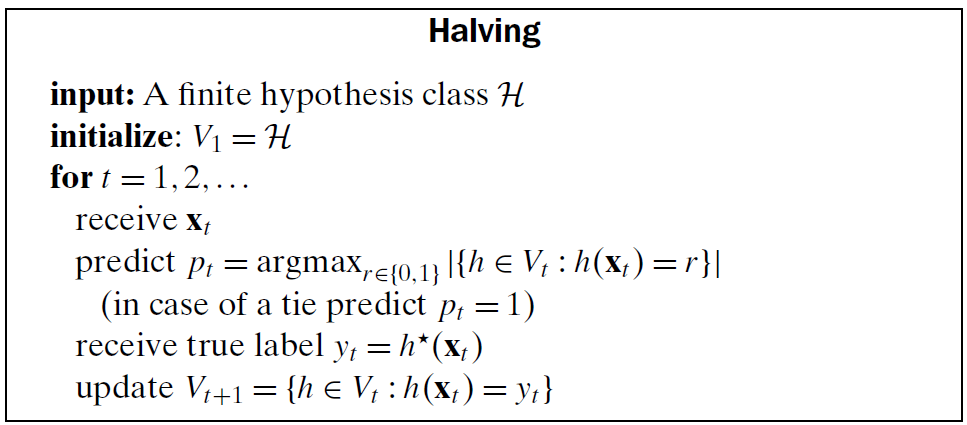
\includegraphics[width=0.8\textwidth]{./figures/Halving.png}
\end{figure}

\pause

\begin{thm}
Let H be a finite hypothesis class. The Halving algorithm enjoys the mistake bound:
\begin{equation}
\Myp_{\mathrm{Halving}}(\Hyp) \leq \log_2(|\Hyp|)
\end{equation}
\end{thm}

\end{frame}
\begin{frame}{Halving}
\begin{proof}
Whenever the algorithm make a mistake, we will simply have:
$$|V_{t+1}| \leq \frac{|V_{t}|}{2}$$
Therefore, if $M$ is the total number of mistakes, we have:
\begin{equation}
1 \leq |V_{T+1}| \leq |\Hyp| 2^{-M}
\end{equation}
\end{proof}
\end{frame}

\begin{frame}{Optimality}
\begin{itemize}
\item 
Learner $\Longleftrightarrow$  Adversary

\pause

\item
Suppose that the environment wants to have the learner make mistake on the all first $T$ rounds of the game.Then, it must output $y_t = 1 - p_t \ \ \forall t \leq T$, and the only question is how it should choose the instances $x_t$ in such a way that ensures that for some $h \in \Hyp$ we have $y_t = h(x_t)$ for all $t$.
\end{itemize}
\end{frame}

\begin{frame}{Littlestone's Dimension}
\begin{figure}[h!]
\centering
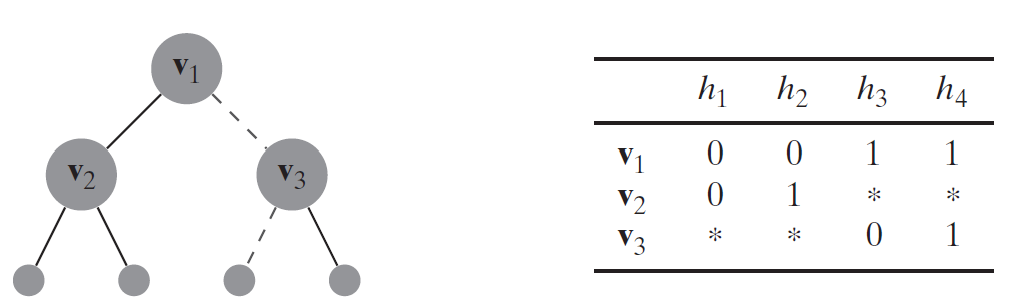
\includegraphics[width=0.8\textwidth]{./figures/Littlestone.png}
\end{figure}

\pause
\begin{itemize}
\item 
A tree of depth $T$
\item
with $2^{T+1} -1$ nodes

\pause
\item
If the learner predicts $p_t=1 \ (p_t= 0)$, the adversary will declare that this is a wrong prediction and $y_t= 0 \ (y_t= 1)$!
and will traverse to the left(right) child of the current node. 
\pause
$\longrightarrow i_{t+1}= 2 i_t+ y_t= 2^{t-1}+ \sum_{j=1}^{t-1}  y_j 2^{t-1-j}$
\end{itemize}
\end{frame}

\begin{frame}{Littlestone's Dimension}
\begin{defs}
A shattered tree of depth $d$ is a sequence of instances $v_1,. . . ,v_{2^d - 1}$ in $\Xspace$ such that for every labeling $(y_1, \hdots, y_d) \in  \{0,1\}^d$ there exists $h \in \Hyp$ such that for all $t \in [d]$ we have $h(v_{i_t}) = y_t$ where $i_{t+1}= 2 i_t+ y_t= 2^{t-1}+ \sum_{j=1}^{t-1}  y_j 2^{t-1-j}$
\end{defs}

We saw a shattered tree of depth 2 in last slide.

\begin{defs}
\textbf{Littlestone’s Dimension ($Ldim$)}: $Ldim(\Hyp)$ is the maximal integer $T$ such that there exists a shattered tree of depth $T$, which is shattered by $\Hyp$.
\end{defs}
\end{frame}


\begin{frame}{Littlestone's Dimension}
\begin{thm}
No  algorithm can have a mistake bound strictly smaller than $Ldim(\Hyp)$. namely, for every algorithm, $\Ayp$, we have 
\begin{equation}
\Myp_\Ayp(\Hyp) \geq Ldim(\Hyp) 
\end{equation}
\end{thm}    

\begin{proof}
Let $T = Ldim(H)$. If the adversary sets $x_t = v_{i_t}$ and $y_t =
1 - p_t$ for all $t \in [T]$, then the learner makes $T$ mistakes while the definition of $Ldim$
implies that there exists a hypothesis $h  \in \Hyp$ such that $y_t = h(x_t)$ for all t. 
\end{proof}

Clearly, We have $Ldim(\Hyp) \leq \log_2 (|\Hyp|)$
\end{frame}

\begin{frame}{Standard Optimal Algorithm}
\begin{figure}[h!]
\centering
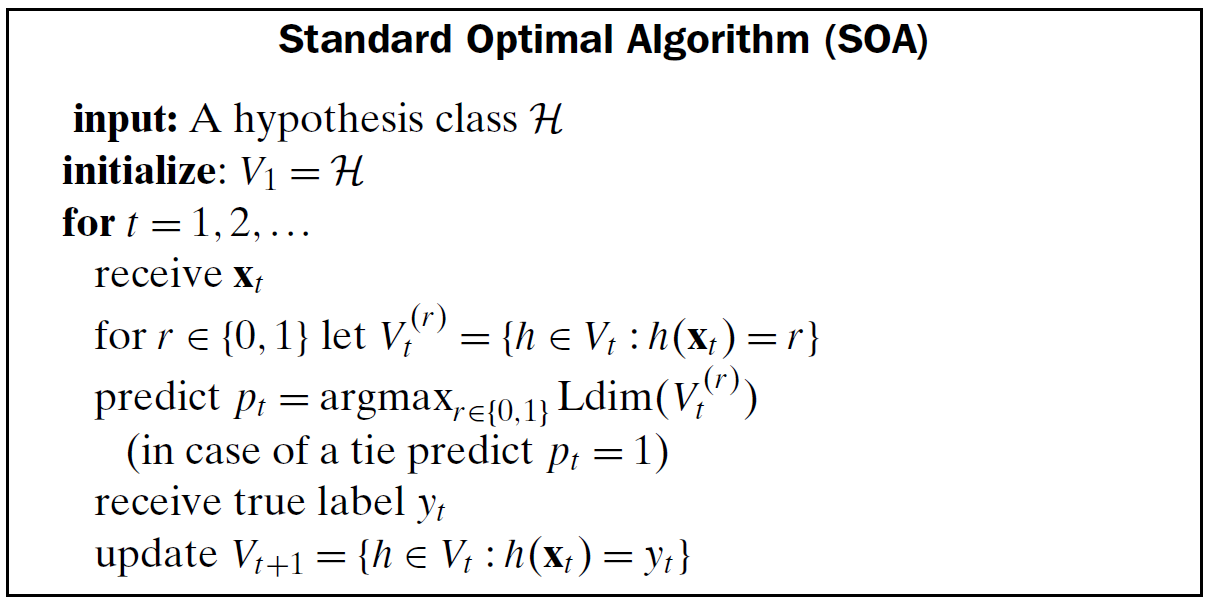
\includegraphics[width=0.7\textwidth]{./figures/SOA.png}
\end{figure}

\begin{thm}
SOA enjoys the mistake bound 
\begin{equation}
\Myp_{\mathrm{SOA}}(\Hyp) \leq Ldim(\Hyp)
\end{equation}
\end{thm}
\end{frame}


\begin{frame}{Standard Optimal Algorithm}
\begin{figure}[h!]
\centering
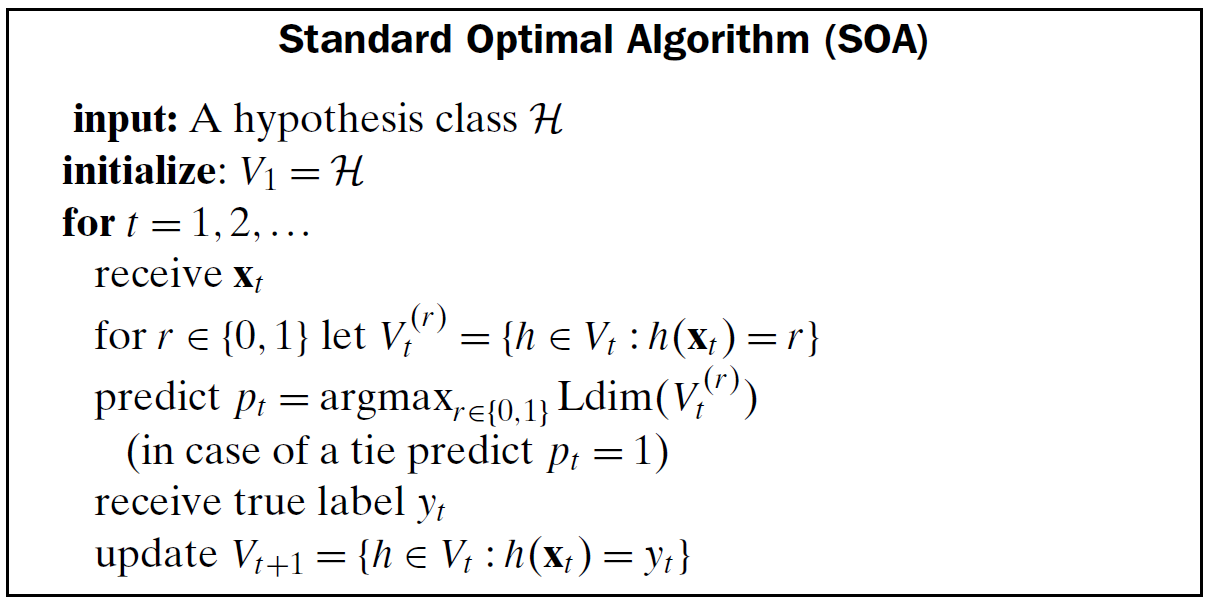
\includegraphics[width=0.7\textwidth]{./figures/SOA.png}
\end{figure}

\begin{proof}
It suffices to show that $Ldim(V_{t+1}) \leq Ldim(V_{t}) -1 $ \\
by contradiction suppose that $Ldim(V_{t+1}) = Ldim(V_{t})$, then will have $Ldim(V_t^{(r)})=  Ldim(V_{t})$ for $r= 0, 1$ which contracts our first assumption!
\end{proof}

\end{frame}

\begin{frame}{Randomization}
\begin{itemize}
\item 
Now suppose there is no such a target function 
$h^*$
and adversary can set loss function whatever it wants, by this we also mean it can change target function in every step!
\item
If the learner was using a deterministic algorithm, it would be pretty unfair because the adversary knew the output every time. So we may want to assume a randomized setting.
\pause
take this problem for example:

$$ l_t(p_t, y_t)= \mathbf{1}\{p_t \neq y_t\}, \ \ p_t, y_t \in \{0, 1\}$$

\pause
obviously enough, adversary sets $y_t=  \Bar{p_t}$ and loss is $1$ all the time!

however if we set $p_t=0$ with probability $\alpha$ and $p_t=1$ otherwise, we have:
\begin{equation}
\mathbb{E}[l_t]= |\alpha- y_t| 
\end{equation}

\end{itemize}
\end{frame}

\begin{frame}{Randomization}
Another important example of randomization that will get back to it:

\begin{figure}[h!]
\centering
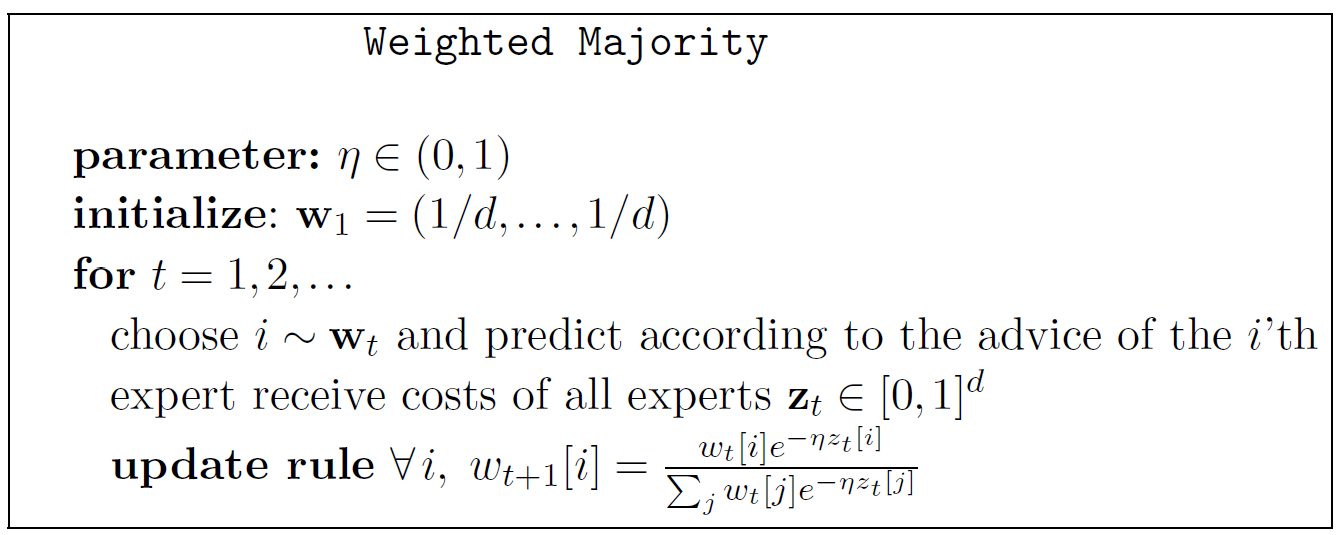
\includegraphics[width=0.7\textwidth]{./figures/Weighted Majority.png}
\end{figure}

\end{frame}


\section{Online Convex Optimization (OCO)}
%\subsection{Basics and Examples}


\begin{frame}
\frametitle{Online Convex Optimization}
\begin{figure}
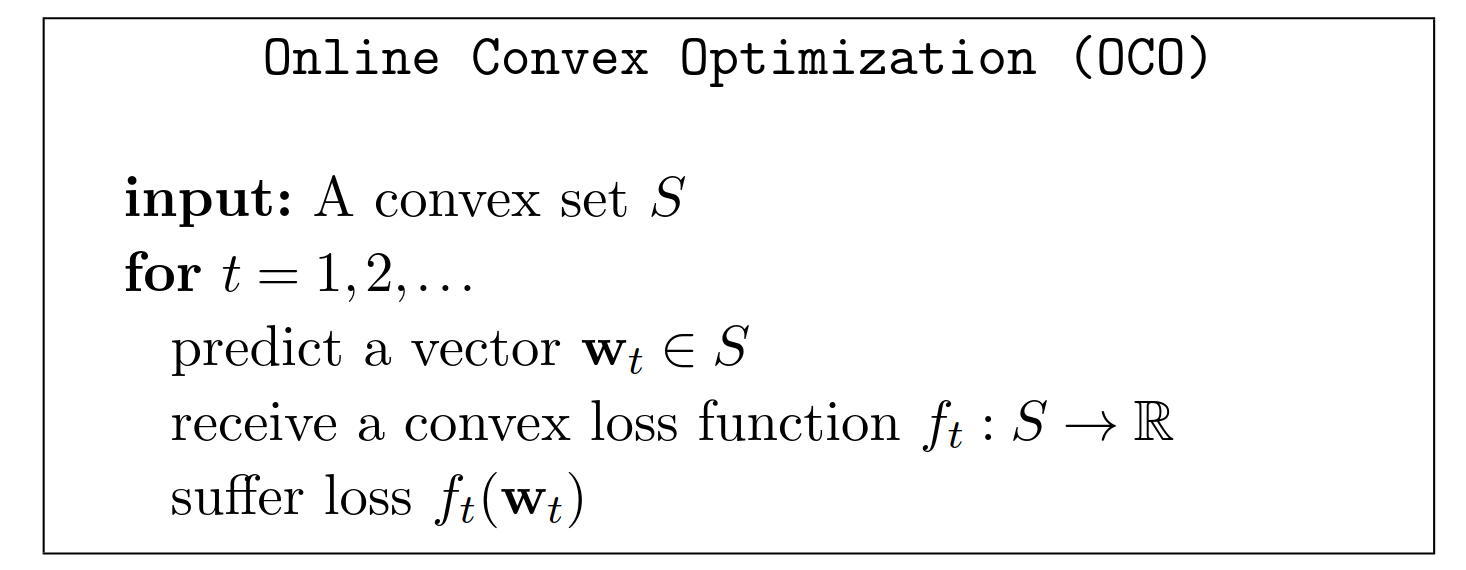
\includegraphics[scale=0.15]{./figures/OCO.png}
\end{figure}

The regret of the algorithm is defined as
\begin{equation}
\mathrm{Regret}_T(\uu) = \sum_{t = 1}^{T} f_t(\w_t) - \sum_{t = 1}^{T} f_t(\uu).
\end{equation}
\end{frame}


\begin{frame}
\frametitle{Examples}
\begin{itemize}
\item \textbf{Convex Optimization:} The adversary plays a fixed $f$:

$$f\big(\frac{1}{T}\sum_{t = 1}^{T}\w_t\big) - f(\w*) \leq \frac{1}{T}\sum_{t=1}^{T} f(\w_t) - \frac{1}{T}\sum_{t=1}^{T} f(\w^*) \leq \frac{\mathrm{Regret}_T(\w^*)}{T}$$

\item \textbf{Online Linear Regression:} This problem is just an example of OCO.
\begin{itemize}
\item Learner receives $\x_t$.
\item Learner decides $\w_t$. 
\item Adversary plays $y_t$.
\item Learner pays the loss $l = |\langle \w, \x_t \rangle - y_t|$
\end{itemize}
\pause
\item Other online prediction problems do not fit into the online convex optimization framework. 
\pause 

\item We will use convexification tricks.
\end{itemize}
\end{frame}


\begin{frame}
\frametitle{Convexification: Randomization}

\begin{itemize}
\item \textbf{Randomization}:
On each round, choose from the advice of $d$ given experts.
\begin{itemize}

\item At round $t$, the learner chooses $\w_t \in S$
\item  An expert $p_t$ is chosen at random according to $\w_t$. 
\item
The cost vector $\y_t$ is revealed.
\pause
\item Expected loss: 

$$\mathbb{E}[y_t[p_t]] = \sum_{i = 1}^{d} \mathbb{P}[p_t = i] y_t[i] = \langle \w_t, \y_t \rangle.$$

\item Note that the adversary does not know the outcome $p_t$; it is random.

\pause 
\item The regret:
\begin{equation*}
\mathrm{Regret}_T(\uu) = \sum_{t = 1}^{T}  \langle \w_t, \y_t \rangle - \langle \w_t, \uu \rangle
\end{equation*}
\end{itemize}
\end{itemize}
\end{frame}


\section{Follow The Leader}

\frame{\sectionpage}

\begin{frame}
\frametitle{Follow the Leader}
The most natural algorithm is Follow-The-Leader (FTL):
\begin{equation*}
\forall t, \;\; \w_t = \argmin_{\w \in S} \sum_{i = 1}^{t-1} f_i(\w)
\end{equation*}
\pause
To analyze FTL, we first prove the following lemma:

\begin{block}{Difference Lemma}
\label{diff_lemma}
Let $\w_1, \w_2, \dots$ be the sequence of vectors produced by FTL. Then, for all $\uu \in S$, we have:
\vspace{-0.4cm}
$$\mathrm{Regret}_T(\uu) = \sum_{t = 1}^{T} \big(f_t(\w_t) - f_t(\uu)\big) \leq \sum_{t = 1}^{T} \big(f_t(\w_t) - f_t(\w_{t+1})\big).$$
\vspace{-0.4cm}
Equivalently, \begin{equation}
\label{eq4}
\sum_{t = 1}^{T} f_t(\w_{t+1}) \leq \sum_{t = 1}^{T} f_t(\uu).
\end{equation}

\end{block}
\end{frame}

\begin{frame}
\frametitle{Follow the Leader}

\begin{block}{Proof}

We prove \eqref{eq4} by induction. The base for $T = 1$ follows from the definition of $\w_{t+1}$. Assume the inequality hold for $T-1$, then for all $\uu \in S$ we have
\vspace{-0.3cm}
\begin{equation}
\label{eq5}
\sum_{t = 1}^{T-1} f_t(\w_{t+1}) \leq \sum_{t = 1}^{T-1} f_t(\uu).
\end{equation}
\vspace{-0.1cm}
\pause
Adding $f_T(\w_{T+1})$ to both sides, we get
\vspace{-0.1cm}
\begin{equation}
\label{eq6}
\sum_{t = 1}^{T} f_t(\w_{t+1}) \leq f_T(\w_{T+1}) + \sum_{t = 1}^{T-1} f_t(\uu).
\end{equation}
\vspace{-0.1cm}
\pause
The above holds for all $\uu$ and in particular for $\uu = \w_{T+1}$. Thus, \vspace{-0.3cm}

\begin{equation}
\label{eq7}
\sum_{t = 1}^{T} f_t(\w_{t+1}) \leq  \sum_{t = 1}^{T} f_t(\w_{T+1}) = \min_{\uu \in S} \sum_{t = 1}^{T} f_t(\uu).
\end{equation}

\end{block}
\end{frame}

\begin{frame}
\frametitle{Online Quadratic Optimization}

Here we prove a regret bound for a subset of OCO in which $S = \R^d$  at each round $t$, we have $f_t (\w) = ||\w - \z_t||_2^2$ for some $\z_t$.
\pause
\begin{itemize}
\item 
$\forall t, \;\; \w_t = \argmin_{\w \in S} \sum_{i = 1}^{t-1} f_i(\w) \implies \w_t = \frac{1}{t-1}\sum_{i=1}^{t-1}\z_i$. 

\vspace{0.2cm}
Note that we can rewrite
$$\w_{t +1} = \frac{1}{t}\left(\z_t + (t-1)\w_t\right),$$
which yields
$$\w_{t+1} - \z_t = \Big(1-\frac{1}{t}\Big)(\w_t - \z_t).$$

\pause
\item Therefore,
\begin{align*}
f_t(\w_t) - f_t(\w_{t+1}) &= \frac{1}{2} ||\w_t - \z_t||^2 - \frac{1}{2} ||\w_{t+1}-\z_t||^2\\ &=\frac{1}{2}\Big(1-\big(1-\frac{1}{t}\big)^2\Big)||\w_t-\z_t||^2 \leq \frac{1}{t} ||\w_t-\z_t||^2.
\end{align*}

\end{itemize}

\end{frame}

\begin{frame}
For the quadratic OCO, we have 
\begin{align*}
f_t(\w_t) - f_t(\w_{t+1}) \leq \frac{1}{t} ||\w_t-\z_t||^2.
\end{align*}
\pause
Let $L = \max_t ||\z_t||$. Since $\w_t$ is the average of $\z_t$, it also holds that $\w_t \leq L$. By the triangle inequality $||\w_t - \z_t|| \leq 2L$. Hence,
$$\sum_{t = 1}^{T} (f_t(\w_t) - f_t)(\w_{t+1})) \leq (2L)^2 \sum_{t=1}^{T}\frac{1}{t} \leq (2L)^2\big(1+\log(T)\big). $$

\pause
Using Lemma 1, we have
\begin{align*}\mathrm{Regret}_T(\uu) = \sum_{t = 1}^{T} \big(f_t(\w_t) - f_t(\uu)\big) &\leq \sum_{t = 1}^{T} \big(f_t(\w_t) - f_t(\w_{t+1})\big)\\
&\leq (2L)^2\big(1+\log(T)\big).
\end{align*}
\end{frame}

\begin{frame}
\frametitle{Follow the Leader}
\begin{itemize}
\item One might wonder if the algorithm always works! \pause  The answer is negative. Consider a 1D online linear optimization: $f_t(w) = z_t w$.
\pause
\item Let $S = [-1, 1]$ and 
\begin{align*}
&z_1 = -0.5\\
&z_t = 1, \; t = 2, 4, \dots\\
&z_t = -1, \; t = 3, 5, \dots
\end{align*}
\item The prediction of FTL will be set to $w_t = 1$ for $t$ odd and $w_t = -1$ for $t$ even. 

\pause
\begin{itemize}
\item The cumulative loss of FTL: $T$.
\item The cumulative loss of the fixed solution $u = 0 \in S$ is $0$.
\end{itemize}
\pause
\item Hence, the regret is $O(T)$!
\pause
\item Intuitively, FTL fails in the above example because its predictions are not stable.

\end{itemize}
\end{frame}



\section{Follow the Regularized Leader}
\frame{\sectionpage}
\begin{frame}
\frametitle{Follow the Regularized Leader}
Follow-the-Regularized-Leader is a natural modification of the basic FTL algorithm.

\begin{equation*}
\forall t, \;\; \w_t = \argmin_{\w \in S} \sum_{i = 1}^{t-1} f_i(\w) + R(\w)
\end{equation*}

\begin{itemize}
\item We now study the regret under strongly convex regularizes.

\end{itemize}
\end{frame}

\begin{frame}
We will now analyze the regret:

\begin{align*}
\mathrm{Regret}_T(\uu) = \sum_{t = 1}^{T} \Big(f_t(\w_t) - f_t(\uu)\Big)
\end{align*}

Running FTRL on $f_1, \dots, f_t$ is equivalent to running FTL on $f_0, \dots, f_T$ where $f_0 = R$. Hence from the Difference Lemma, we have

\begin{align*}
&\sum_{t = 0}^{T} \Big(f_t(\w_t) - f_t({\uu})\Big) \leq \sum_{t = 0}^{T}\Big( f_t(\w_t) - f_t(\w_{t+1})\Big)
\end{align*}
\pause

Rearranging terms, we arrive at:
\begin{align*}
\sum_{t = 1}^{T} \Big(f_t(\w_t) - f_t({\uu})\Big) \leq R(\uu) - R(\w_1) + \sum_{t = 1}^{T}\Big( f_t(\w_t) - f_t(\w_{t+1})\Big)
\end{align*}
\end{frame}



\begin{frame}
\frametitle{Strongly Convex Regularizers}

We will now analyze FTRL with strongly convex regularizers.

\begin{align*}
\mathrm{Regret}_T(\uu) &\leq R(\uu) - R(\w_1) + \sum_{t = 1}^{T}\Big( f_t(\w_t) - f_t(\w_{t+1})\Big)\\
&\leq R(\uu) - R(\w_1) + \sum_{t = 1}^{T}L ||\w_t - \w_{t+1}||
\end{align*}

So we need to ensure $||\w_t - \w_{t+1}||$ is small.
\end{frame}

\begin{frame}
Let $F_t = \sum_{i = 1}^{t-1} f_i(\w) + R(\w)$ and note that $\w_t = \argmin_{\w \in S} F_t(\w)$.

Since $\w_t$ is the minimizer, by the strong convexity property we have

$$F_t(\w_{t+1})\geq F_t(\w_t) + \frac{\sigma}{2} ||\w_t - \w_{t+1}||^2$$

Reteating the same argument for $F_{t+1}$ and minimizer $\w_{t+1}$:

$$F_{t+1}(\w_{t})\geq F_{t+1}(\w_{t+1}) + \frac{\sigma}{2} ||\w_t - \w_{t+1}||^2$$

\pause
Summing the above inequalities and using Lipschitzness of $f_t$:

$$\sigma||\w_t - \w_{t+1}||^2 \leq f_t(\w_t) - f_t(\w_{t+1}) \leq L||\w_t - \w_{t+1}||$$

This implies

$$||\w_t - \w_{t+1}||^2 \leq \frac{L}{\sigma}.$$
\end{frame}


\begin{frame}
\begin{align*}
\mathrm{Regret}_T(\uu) &\leq R(\uu) - R(\w_1) + \sum_{t = 1}^{T}\Big( f_t(\w_t) - f_t(\w_{t+1})\Big)\\
&\leq R(\uu) - R(\w_1) + \sum_{t = 1}^{T}L ||\w_t - \w_{t+1}||\\
& \leq R(\uu) -\min R + TL^2/\sigma 
\end{align*}
\end{frame}



\begin{frame}
\frametitle{Euclidean Regularization}

\begin{block}{Corollary}

Let $f_1, \dots, f_T$ be a sequence of convex and $L$-Lipschitz functions with respect to $||.||_2$. FTRL is run on the sequence with $R(\w) = \frac{1}{2\eta}||\w||_2^2$.

$$\forall \uu:\;\; \mathrm{Regret}_T(\uu) \leq \frac{1}{2\eta}||\uu||_2^2 + \eta TL^2.$$

In particular, if $U=\{\uu: ||\uu||_2\leq B\}$
and $\eta = \frac{B}{L\sqrt{2T}}$, then

$$\mathrm{Regret}_T(U) \leq BL\sqrt{2T}.$$

\end{block}
\end{frame}


\begin{frame}
\frametitle{Expert Advise}

\begin{block}{Corollary}
Assume that the conditions of the previous corollary hold. Let $S$ be a convex set. Define

$$R(\w) = \begin{cases}
\frac{1}{2\eta}||\w||_2^2& \w \in S\\	\infty& \w \notin S\\
\end{cases}$$

Then 
$\forall \uu \in S:\;\; \mathrm{Regret}_T(\uu) \leq \frac{1}{2\eta}||\uu||_2^2 + \eta TL^2.$

In particular, if $B\geq \max_{\uu \in S} ||\uu||_2$ and $\eta = \frac{B}{L\sqrt{2T}}$, then

$$\mathrm{Regret}_T(S) \leq BL\sqrt{2T}.$$

\end{block}
\pause
In the expert advice setting,  $S$ is the probability simplex and $\x_t \in [0, 1]^d$. We can set $L = \sqrt{d}$ and $B = 1$ which leads to a regret bound $\sqrt{2dT}$.
\pause

The Entropic Regularization leads to $\sqrt{2\log(d)T}$
\end{frame}




\section{Online Mirror Descent}
\frame{\sectionpage}
\begin{frame}
\frametitle{Online Mirror Descent}
\begin{itemize}
\item FTRL involves solving an optimization in each round.
\item We will show that Online Mirror Descent achieves the same regret bound as FTRL

\item
It is capable of introducing a variety of new algorithms 

\item Notation: $z_{1:t} = \sum_{i = 1}^{t} \z_i$.

\end{itemize}
\end{frame}


\begin{frame}{General OMD settings}
\begin{figure}[h!]
\centering
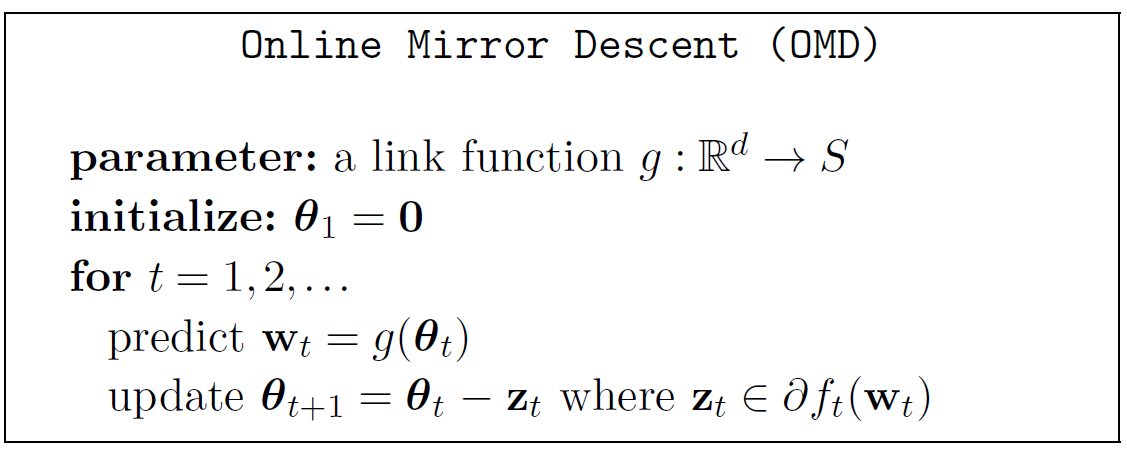
\includegraphics[width=0.6\textwidth]{./figures/OMD.png}
\end{figure}

\begin{itemize}
\item 
Choosing different $g$'s leads to differnet algorithms

\item
For instance, taking $g(x)= x$ results in OGD.

\item
$\theta$ is updated by subtracting the gradient out of it, but the actual prediction is “mirrored” or “linked” to the set $\mathrel{S}$ via the function $g$.

\pause

\item
We will show that it is \textbf{equivalent to FTRL} for some specific regularization.
\end{itemize}

\end{frame}


\begin{frame}

If $f_t$ are convex nonlinear functions, we have
$$\sum_{t = 1}^{T} f_t(\w_t) - f_t(\uu)  \leq \sum_{t = 1}^{T} \langle \w_t - \uu, \z_t \rangle$$

So from now, we will consider the OLO problem.


\pause
Consider the FTRL update:
\vspace{-0.5cm}
\begin{align*}
\w_{t+1} &= \argmin R(\w) + \sum_{i = 1}^{t} \langle \w, \z_t\rangle\\
&= \argmin R(\w) + \langle \w, \z_{1:t} \rangle\\
&= \argmax - R(\w) + \langle \w, -\z_{1:t} \rangle\\
\end{align*}


\pause
\vspace{-0.5cm}
Let $g(\theta)  = \argmax_\w \langle \w, \theta \rangle - R(\w)$, we can write FTRL as the following recursive rule:

\begin{equation*}
\begin{cases}

\w_{t} = g(\theta_{t})\\
\theta_{t+1} = \theta_{t} - \z_t\\
\end{cases}
\end{equation*}
\end{frame}



\subsection{Regret Analysis}
\begin{frame}{Preliminaries}
\begin{block}{Reminder}

\begin{itemize}
\item \textbf{Conjugate function}:

$$f^*(\theta) = \max_\uu \langle \uu, \theta \rangle - f(\uu).$$

\item \textbf{Fenchel-Young's Inequality}:

$$\forall \uu, \;\; f^*(\theta)+ f(\uu) \geq \langle \uu, \theta \rangle$$

\item \textbf{Bregman's Divergence}: A differentiable convex function $R$ defines a Bregman divergence between two vectors as follows:

$$D_R (\w||\uu) = R(\w) - \big(R(\uu) + \langle \nabla R(\uu), \w - \uu\rangle\big) \geq 0$$

For example $R(w)= \frac{1}{2} ||w||_2^2$ gives $D_R (\w||\uu)= ||w- u||_2^2$ and $R(w)= \sum_i w[i] \log(w[i])$
gives KL-divergence.




\end{itemize}
\end{block}
\end{frame}

\begin{frame}{Preliminaries}


\begin{figure}
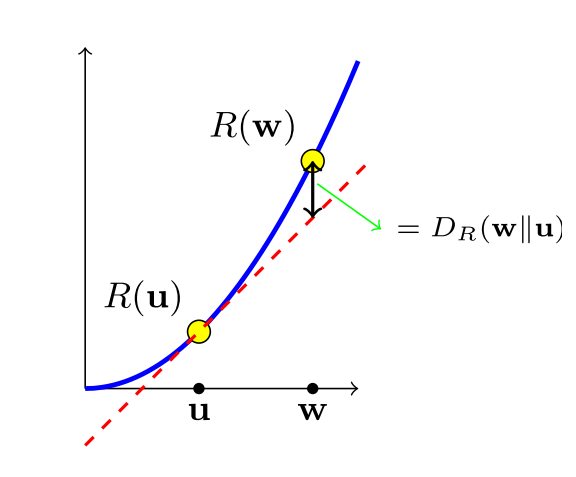
\includegraphics[scale=0.25]{./figures/bregman.png}
\end{figure}


\end{frame}



\begin{frame}{Preliminaries}

\begin{itemize}
\item \textbf{Strong-Convexity}:

$$D_R(\w|| \uu) \geq \frac{\sigma}{2}||\w-\uu||^2.$$

\item \textbf{Strong-Smoothness}:
$$D_R(\w|| \uu) \leq \frac{\sigma}{2}||\w-\uu||^2.$$

\pause

\begin{lem}
(Strong/Smooth Duality) Assume that $R$ is a closed and convex function. Then $R$ is $\beta$-strongly convex with respect to a norm $||.||$ if and only if $R^*$ is $\frac{1}{\beta}$-strongly smooth with respect to the dual norm $||.||_*$
\end{lem}



\end{itemize}
\end{frame}


\begin{frame}{Preliminaries}
\begin{lem}
It is possible to show that equality in Fenchel-Young Inequality holds if $u$ is a sub-gradient of
$f^*$ at $\theta$ and in particular, if $f^*$ is differentiable, equality holds when $\uu= \nabla f^* (\theta)$. In the same way, $\theta = \nabla f(u)$
\end{lem}


\pause


Recall that $g(\theta)  = \argmax_\w \langle \w, \theta \rangle - R(\w)$. then:

\begin{equation}
g(\theta)= \nabla R^*(\theta)
\end{equation}


\end{frame}


\begin{frame}
\frametitle{Analysis of OMD}

\begin{lem}
Suppose that OMD is run with a link function $g(\theta)= \nabla R^*(\theta)$
Then, its regret is upper bounded by:

\begin{equation}
\sum_{t=1}^T  \langle w_t-\uu , z_t \rangle \leq  R(\uu)-R(w_1)+  \sum_{t=1}^T D_{R^*}(-z_{1:t}|| -z_{1:t-1}).
\end{equation}
\end{lem}


\end{frame}



\begin{frame}
\frametitle{Analysis of OMD}



\begin{proof}
Using Fenchel–Young inequality we have:
{\scriptsize
$$R(\uu)+ \sum_{t=1}^T  \langle \uu , z_t \rangle=  R(\uu)- \langle \uu , -z_{1:T} \rangle \geq -R^*(-z_{1:T})$$
}

\pause

\vspace{-0.2cm}
if we rewrite the RHS as: 
{\scriptsize
$$-R^*(-z_{1:t})= -R^*(0)- \sum_{t=1}^T (R^*(-z_{1:t}) -R^*(-z_{1:t-1}))$$
}
\vspace{-0.2cm}

\pause

knowing that $w_t=  \nabla R^*(-z_{1:t-1})$:
{\scriptsize
$$=  -R^*(0)+ \sum_{t=1}^T (\langle  w_t, z_t \rangle - D_{R^*}(-z_{1:t} ||-z_{1:t-1}))$$
}
\vspace{-0.2cm}

Note that $R^*(\mathbf{0})= max_w \{\langle \mathbf{0}, w \rangle- R(w)\}= - min_w\{R(w)\}= -R(w_1)$

Combining all the above concludes the proof.

\end{proof}

\end{frame}


\begin{frame}{Analysis of OMD}
\begin{block}{Corollary}
Let R be a $\frac{1}{\eta}$-strongly convex with respect to a norm $||.||$ and suppose the OMD algorithm is run with the link function $g= \nabla R^*$, Then:
$$\sum_{t=1}^T  \langle w_t-\uu , z_t \rangle \leq  R(\uu)-R(w_1)+   \frac{\eta}{2} \sum_{t=1}^T ||z_t||_*^2$$
\end{block}

That is what we had for OGD, which is reassuring

\end{frame}


\subsection{Normalized Exponentiated Gradient}
\begin{frame}
\frametitle{Derived Algorithms}
\framesubtitle{Normalized Exponentiated Gradient}
Let $S$ be the probability simplex and $g: \R^d \to \R^d$ be a vector valued function whose i'th component is 
$$g_i(\theta) = \frac{\exp(\eta\, \theta[\,i\,])}{\sum_j\exp(\eta \,\theta[\,j\,])}  \iff R(\w) = \frac{1}{\eta}\sum_{i} w[\,i\,] \log(w[\,i\,]) \text { on } S$$


The update of OMD with this function is 
$$w_{t+1}[
\,i\, ] = \frac{w_t[\, i\,] \exp(-\eta z_t[\, i\,])}{\sum_{j} w_t[\, j\,] \exp(-\eta z_t[\, j\,])}$$

\pause

\begin{thm}
Assume that the normalized EG algorithm is run on a sequence of linear loss functions such that for all $t, i$ we have $\eta z_t[i] \geq -1$.
Then:

\begin{equation}
\sum_{t=1}^T  \langle w_t-\uu , z_t \rangle \leq \frac{\log(d)}{\eta}  + \eta \sum_{t=1}^T \sum_i w_t[i] z_t[i]^2
\end{equation}

\end{thm}

\end{frame}




\begin{frame}

\begin{block}{proof.}
it suffices to show that:
\vspace{-0.2cm}

$$D_{R^*}(-z_{1:t}|| -z_{1:t-1}) \leq   \eta    \sum_i w_t[i] z_t[i]^2$$

\vspace{-0.3cm}


\pause

the conjugate function of $R(\w) = \frac{1}{\eta}\sum_{i} w[\,i\,] \log(w[\,i\,])$ is:
\vspace{-0.2cm}


$$R^*(\theta)= \frac{1}{\eta}  \log(\sum_i e^{\eta \theta[i]})$$
\vspace{-0.3cm}

\pause

then:
\begin{align*}
D_{R^*}(-z_{1:t}|| -z_{1:t-1}) & = -R^*(-z_{1:t})- R^*(-z_{1:t-1}) +  \langle w_t, z_t \rangle \\
& = \frac{1}{\eta}  \log(\frac{ \sum_i e^{- \eta z_{1:t}[i]} }{ \sum_i e^{- \eta z_{1:t-1}[i]} })+ \langle w_t, z_t \rangle \\
&=  \frac{1}{\eta}  \log(\sum_i  w_t[i] e^{-\eta z_{t}[i]} )+ \langle w_t, z_t \rangle
\end{align*}

\end{block}

\end{frame}





\begin{frame}

\begin{block}{proof.}
Using numeric inequality: $e^{-a} \leq 1-a+a^2 \,  a\geq -1$, we obtain:
$$D_{R^*}(-z_{1:t}|| -z_{1:t-1}) \leq \frac{1}{\eta}  \log(\sum_i  w_t[i] (1 -\eta z_{t}[i] + \eta^2 z_{t}[i]^2))+ \langle w_t, z_t \rangle$$


\pause

and the inequality $\log(1 - a) \leq  -a$,

\begin{align*}
D_{R^*}(-z_{1:t}|| -z_{1:t-1}) & \leq \frac{1}{\eta}  \sum_i  w_t[i] ( -\eta z_{t}[i] + \eta^2 z_{t}[i]^2)+ \langle w_t, z_t \rangle \\
& =  \eta  \sum_i  w_t[i] z_{t}[i]^2
\end{align*}


\end{block}

\end{frame}




\subsection{$L_p$ Algorithm}
\begin{frame}
\frametitle{Derived Algorithms}
\framesubtitle{$L_p$ Algorithm}
Let $g: \R^d \to \R^d$ be a vector valued function with 
{\scriptsize
$$g_i(\theta) = \eta \frac{\mathrm{sign}(\theta[\, i\,]) \Big|\theta[\, i\,]\Big|^{p-1}}{||\theta||_p^{p-2}}$$
}

$g(\theta)$ is the update corresponding to  $R(\w) = \frac{1}{2\eta (q-1)}||\w||_q^2$ where $\frac{1}{p} + \frac{1}{q} = 1$ and $R$ is $\frac{1}{\eta}$-strongly convex with respect to $l_q$ norm.

\begin{block}{Corollary}
Let $f_1, \dots, f_T$ be a sequence of convex and $L$-Lipschitz function over $\R^d$ with respect to $||.||_q$. Then for all $\uu$ for the $L_p$ algorithm we have

\vspace{-0.3cm}
{\small$$\mathrm{Regret}_T(\uu) \leq \frac{1}{2\eta(q-1)}||\w||_q^2 + \eta T L^2$$}
\end{block}

\pause
If $||\uu||_q \leq B$ and $\eta = \frac{B}{L\sqrt{2T/(q-1)}}$ then $\mathrm{Regret}_T(U) \leq BL\sqrt\frac{2T}{q-1}$.
\end{frame}



\section{Bandits}
\frame{\sectionpage}


\begin{frame}
In this section:

\begin{enumerate}
\item Review
\item Multi-Armed Bandits (Adversarial)
\begin{enumerate}
\item Multi-Armed Bandits Algorithm
\end{enumerate}
\item Multi-Armed Bandits (Stochastic)
\begin{enumerate}
\item Explore-Then-Commit
\item Upper Confidence Bound
\end{enumerate}

\end{enumerate}
\end{frame}

\begin{frame}
\frametitle{Bandits: Introduction}
What we have done so far:
\pause

\begin{itemize}
\item \textbf{Online Convex Optimization}

\begin{figure}
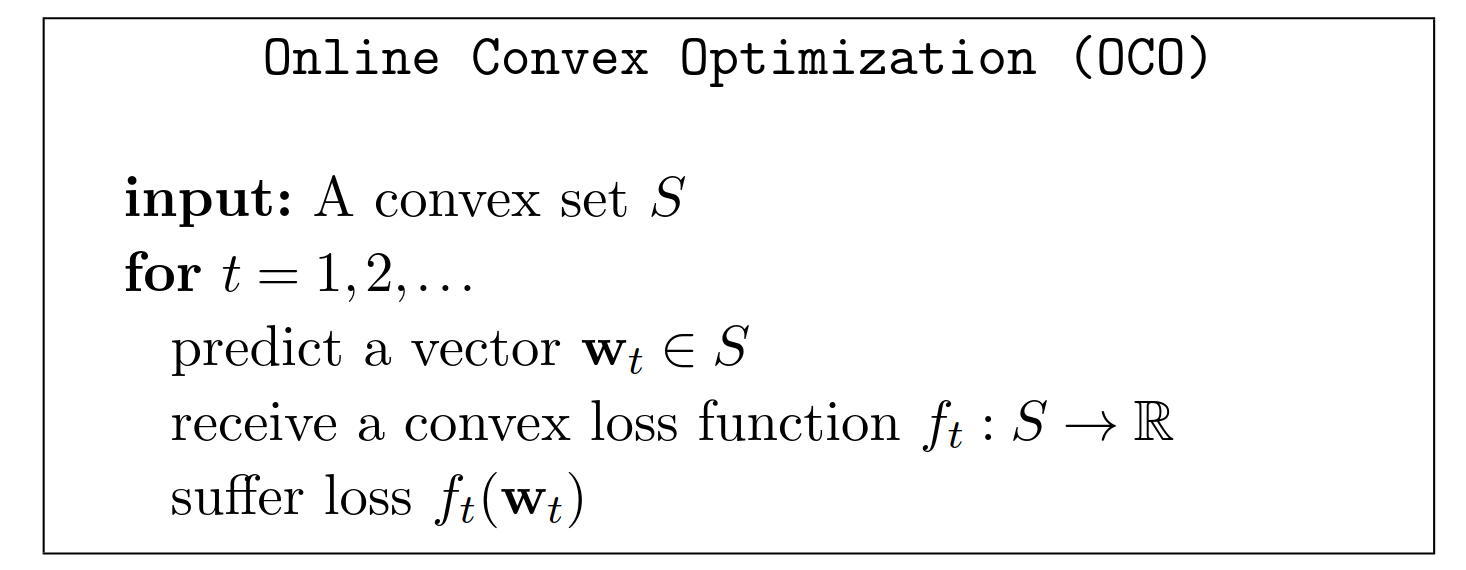
\includegraphics[scale=0.15]{./figures/OCO.png}
\end{figure}

\end{itemize}
\end{frame}



\begin{frame}{Limited Feedback (Bandits)}
\begin{itemize}
\item Recall the OMD algorithm we described in last section. 

\begin{figure}[h!]
\centering
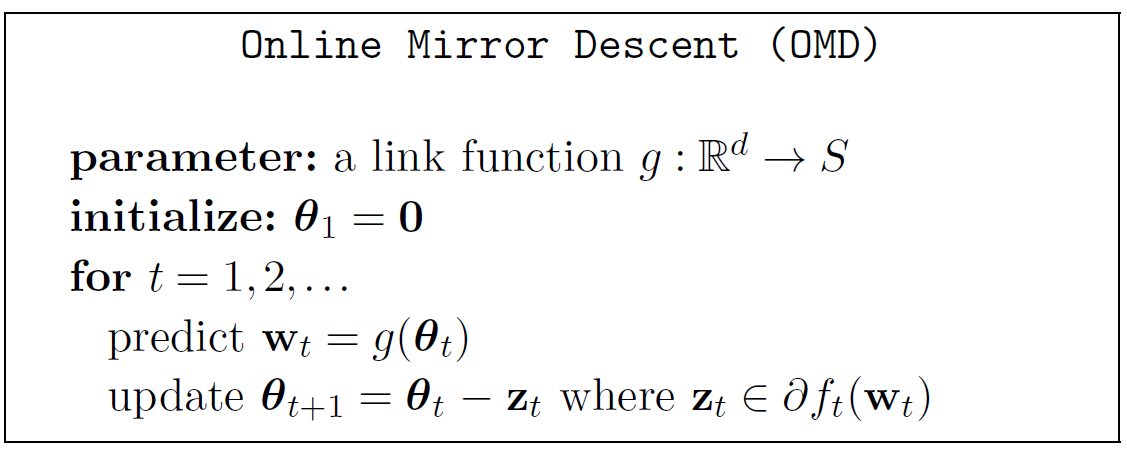
\includegraphics[width=0.6\textwidth]{./figures/OMD.png}
\end{figure}

\item What if we won't be given $\z_t$ after each step? 

\pause

Remember $z_t$ was, For instance, in case of linear loss, vector constructed by expert's losses! 

\pause

\item 
Therefor, It's natural to assume that we are just given $\z_t[i]$
with probability $\w_t[i]$.
\end{itemize}
\end{frame}



\begin{frame}
\begin{center}
{\Large Bandit $\equiv$ Limited Feedback}

\pause \vspace{2cm}

The learner knows $f_t(\w_t)$ but not the function $f_t$ or its drrivative $\z_t \in \partial f_t(\w_t)$.

\end{center}
\end{frame}


\begin{frame}{Limited Feedback (Bandits)}
\begin{itemize}
\item
An unbiased estimator of $z_t$ might suffices.

\pause

\begin{figure}[h!]
\centering
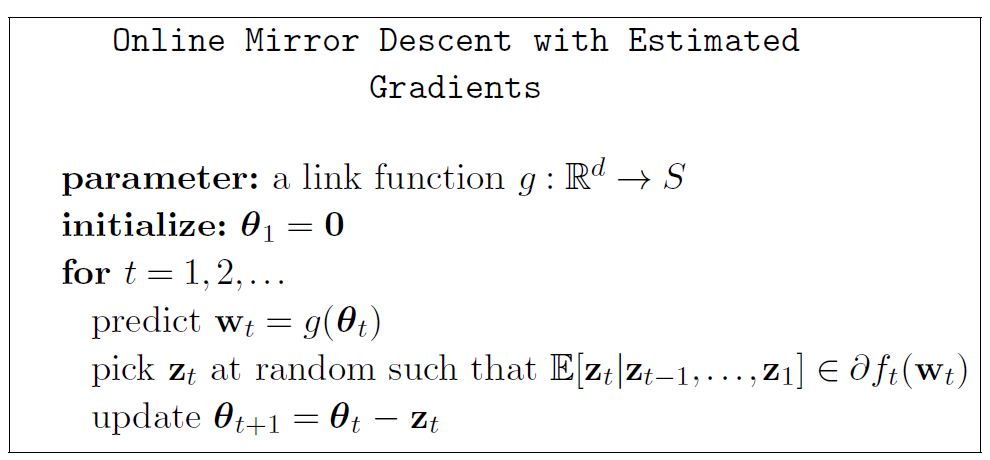
\includegraphics[width=0.7\textwidth]{./figures/Bandit.png}
\end{figure}


\end{itemize}
\end{frame}


\begin{frame}{Limited Feedback (Bandits)}
\begin{thm}
Suppose that the estimated sub-gradients are chosen such that with probability 1 we have:
$$ \sum_{i=1}^T \langle \w_t - \uu, \z_t \rangle \leq B(\uu) + \sum_{i=1}^T ||\z_t||_t^2$$

where $B$ is some function, and for all round $t$ the norm $||.||_t$ may depend on $w_t$. Then:
$$\mathbb{E}[\sum_{i=1}^T f_t(\w_t)- f_t(\uu)] \leq B(\uu) + \sum_{i=1}^T \mathbb{E}[||\z_t||_t^2]$$

Where the expectation is with respect to the randomness in choosing $\z_1, \dots, \z_T$.
\end{thm}

\end{frame}



\begin{frame}{Limited Feedback (Bandits)}
\begin{proof}
Taking expectation of both sides with respect to the randomness in choosing $\z_t$:

$$ \mathbb{E}\Big[\sum_{i=1}^T \langle \w_t - \uu, \z_t \rangle\Big]  \leq B(\uu) + \sum_{i=1}^T \mathbb{E}\big[||\z_t||_t^2\big]$$

By the law of total probability $\Big(\vv_t = \mathbb{E}[\z_t|\z_{t-1}, \dots, \z_1] \in \partial f_t(\w_t)\Big)$:

$$\mathbb{E}\big[\sum_{i=1}^T \langle \w_t - \uu, \z_t \rangle\big]= \mathbb{E}\big[\sum_{i=1}^T \langle \w_t - \uu, \vv_t \rangle\big]$$

\pause

Due to the convexity we also know that: 

$$ \langle \w_t - \uu, \vv_t \rangle \geq f_t(\w_t)- f_t(\uu) $$
\end{proof}


we may come to the conclusion that by using an estimation of the sub-gradient all previous results remains true for expectation of the Regret. But we have not seen everything yet!
\end{frame}


\subsection{Multi-Armed Bandits}
\frame{\subsectionpage}


\begin{frame}
\frametitle{Multi-Armed Bandits (MAB)}

A natural bandit version of Learning from Expert Advice (LEA):


\begin{figure}[h!]
\centering
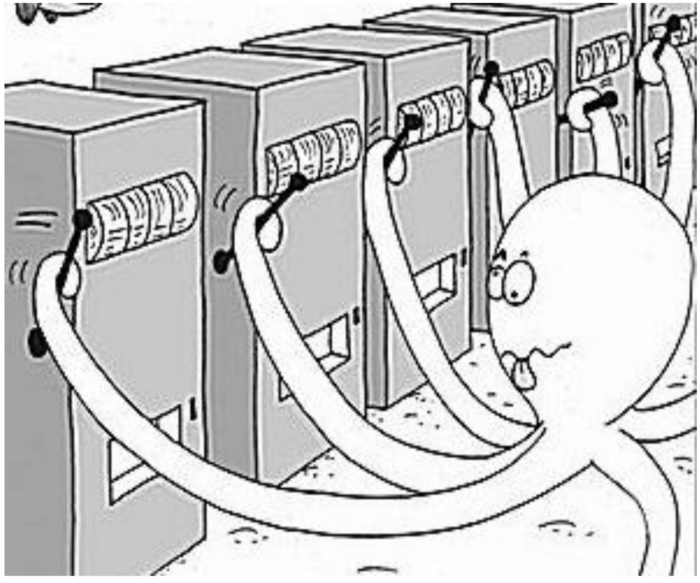
\includegraphics[width=0.4\textwidth]{./figures/MAB.png}
\end{figure}

\pause

\begin{center}
Exploration vs. Exploitation
\end{center}

\end{frame}



\begin{frame}{Multi-Armed Bandit}
\begin{itemize}
\item
The vector $\y_t \in  [0, 1]^d$ associates a
cost for each of the arms, but the learner only gets to see the cost
of the arm it pulls.

\pause
\item The goal is to have low regret:

$$\mathbb{E}\Big[\sum_{t=1}^T \y_t[p_t]\Big] - \underset{i}{\mathrm{\min}} \sum_{t=1}^T \y_t[i] $$   

\end{itemize}

\end{frame}


\begin{frame}{Multi-Armed Bandit}

\begin{itemize}
\item Let $S$ be the probability simplex.
\item 	The learner picks an arm according to $\mathbb{P}[p_t = i] = \w_t[i]$ and therefore $f_t(\w) = 	\langle \w , \y_t \rangle$ is the expected cost of the chosen arm.


\item 
To estimate the gradient:

$$\z_t [\,j\,]=  \begin{cases}
\frac{y_t[\,j\,]}{w_t[\,j\,]} &  j=p_t\\
0             & \text{else}
\end{cases}
$$

$$ \mathbb{E}\big[\z_t^{(p_t)}[\,j\,]| \z_{t-1}, \hdots, z_1\big]= \sum_{i=1}^d \mathbb{P}[\,p_t = i\,] z_t^{(i)}[\,j\,]= w_t[\,j\,] \frac{y_t[\,j\,]}{w_t[\,j\,]}= y_t[\,j\,]$$
\end{itemize}    
\end{frame}


\begin{frame}{Multi-Armed Bandit}



if we update $\w_t$ using the update rule of the normalized EG algorithm we saw before:

\begin{figure}[h!]
\centering
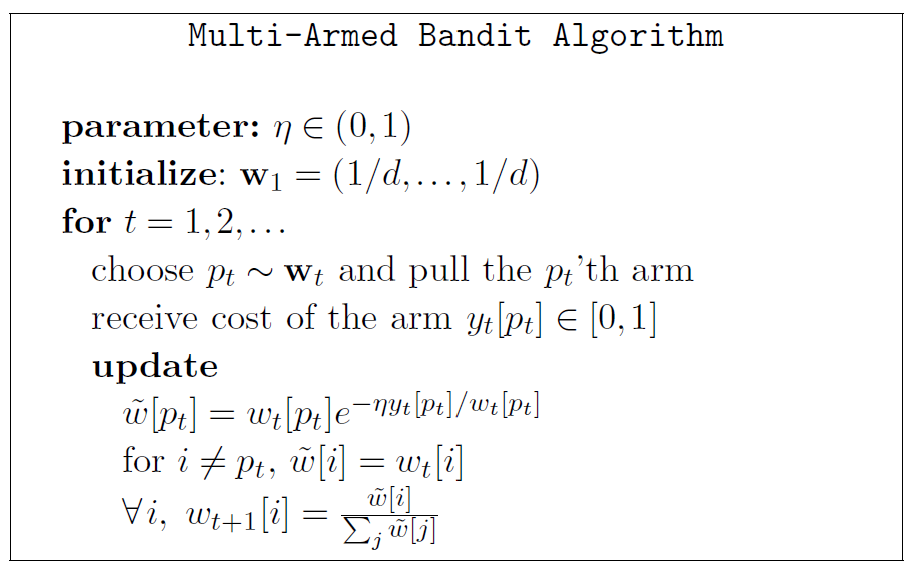
\includegraphics[width=0.6\textwidth]{./figures/Multi_armed.png}
\end{figure}

\end{frame}

\begin{frame}{Multi-armed bandit}
For the exponentiated gradient, we proved that:
$$\sum_{t=1}^T  \langle w_t-\uu , z_t \rangle \leq \frac{\log(d)}{\eta}  + \eta \sum_{t=1}^T \sum_i \w_t[i] \z_t[i]^2$$

\pause\vspace{-0.2cm}
Thus,
$$\mathbb{E}\Big[\sum_{i=1}^T f_t(\w_t)- f_t(\uu)\Big] \leq \frac{\log(d)}{\eta}  + \eta \sum_{t=1}^T \sum_i \mathbb{E}[\w_t[i] \z_t[i]^2]$$

\pause

The last term can be bounded as:
\begin{align*}
\mathbb{E}\Big[\sum_i\w_t[\,i\,] \z_t^{(p_t)}[\,i\,]^2 \Big| \z_{t-1}, \hdots, \z_1\Big] &=  \sum_j \mathbb{P}[\,p_t= j\,] \sum_i \w_t[\,i\,] \z_t^{(j)}[\,i\,]^2\\
&=  \sum_j \w_t[\,j\,] \w_t[\,j\,] \Big(\frac{\y_t[\,j\,]}{\w_t[\,j\,]}\Big)^2\\
&= \sum_j \y_t[\,j\,]^2 \leq d
\end{align*}

\end{frame}


\begin{frame}{Multi-armed bandit} 
\begin{block}{Corollary}

The multi-armed bandit algorithm enjoys the bound
$$\mathbb{E}\Big[\sum_{t=1}^T y_t[p_t]\Big] \leq  \underset{i}{\mathrm{min}} \sum_{t=1}^T y_t[i]+ \frac{\log(d)}{\eta}+ \eta dT.$$

In particular, $\eta= \sqrt{\frac{\log(d)}{dT}}$ gives the regret bound $2\sqrt{d\log(d) T}$.


\end{block}



\pause 

There exists a matching lower bound and $\sqrt{d\log(d)}$ is tight.

\end{frame}



\subsection{Stochastic Bandits}
\frame{\subsectionpage}

\begin{frame}{Stochastic Bandits}
\begin{itemize}
\item Each arm $i \in \{1, 2, \dots, d\}$ is a probability distribution $D_i$.
\pause

\item At time $t$, we select arm $A_t$ and receive $\mathbf{g}_{t, A_t} \sim D_{A_t}$.

\pause
\item The Pseudo-Regret is defined as follows:

$$\mathrm{Regret}_T = \mathbb{E}\Big[\sum_{t = 1}^{T}\mathbf{g}_{t, A_t}\Big] - \min_i \mathbb{E}\Big[\sum_{t = 1}^{T}\mathbf{g}_{t, i}\Big]$$
\end{itemize}
\end{frame}


\begin{frame}{Explore-Then-Commit Algorithm}

The most basic algorithm:
\begin{figure}
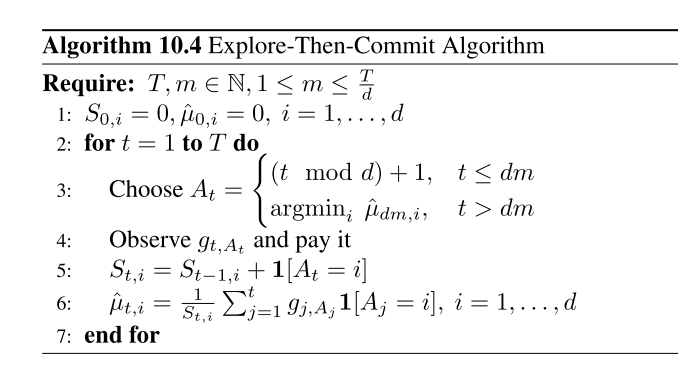
\includegraphics[scale=0.35]{./figures/explore.png}
\end{figure}

\end{frame}


\begin{frame}{ETC: Analysis}

\begin{itemize}
\item $S_{t, i} = \sum_{j=1}^{d}1[A_t = i]$.

\item $\Delta_i = \mu_i - \mu^*$.

\end{itemize}

\begin{lemma}
\label{lemma:stoch_band_decomp}
For any policy of selection of the arms,
\[
\mathrm{Regret}_T = \sum_{i=1}^d \mathbb{E}[S_{T,i}]. \Delta_i~.
\]
\end{lemma}
%

\end{frame}


\begin{frame}{ETC: Analysis}
\begin{proof}
\vspace{-0.7cm}
\begin{small}

\begin{align*}
\mathrm{Regret}_T 
&= \mathbb{E}\left[\sum_{t=1}^T g_{t,A_t}\right] - T \mu^\star 
= \mathbb{E}\left[\sum_{t=1}^T (g_{t,A_t}- \mu^\star)\right] 
\\
&= \sum_{i=1}^d \sum_{t=1}^T \mathbb{E}\Big[\boldsymbol{1}[A_t=i](g_{t,i}-\mu^\star)\Big] = \sum_{i=1}^d \sum_{t=1}^T \mathbb{E}\Big[\mathbb{E}\big[\boldsymbol{1}[A_t=i](g_{t,i}- \mu^\star)|A_t\big]\Big] \\
&= \sum_{i=1}^d \sum_{t=1}^T \mathbb{E}\Big[\boldsymbol{1}[A_t=i] \mathbb{E}\big[g_{t,i} - \mu^\star |A_t\big]\Big] 
\\
&= \sum_{i=1}^d \sum_{t=1}^T \mathbb{E}\Big[\boldsymbol{1}[A_t=i] (\mu_{A_t}- \mu^\star)\Big] 
= \sum_{i=1}^d \sum_{t=1}^T \mathbb{E}\big[\boldsymbol{1}[A_t=i]\big] (\underbrace{\mu_i- \mu^\star}_{\Delta_i})~.
\end{align*}
\pause


\end{small}

\end{proof}

In order to have a small regret we have to select the suboptimal arms less often then the best one.

\end{frame}


\begin{frame}
\frametitle{ETC: Analysis}
\begin{theorem}
Assume that the losses of the arms minus their expectations are $1$-subgaussian and $1\leq m \leq T/d$. Then, ETC guarantees a regret of
\[
\mathrm{Regret}_T
\leq m \sum_{i=1}^d \Delta_i + (T-md)\sum_{i=1}^d \Delta_i \exp\left(-\frac{m \Delta^2_i}{4}\right)~.
\]
\end{theorem}

\end{frame}

\begin{frame}
\frametitle{ETC: Proof}
\begin{proof}
Let's assume without loss of generality that the optimal arm is the first one. So, for $i\neq 1$, we have
\begin{align*}
\sum_{t=1}^T \mathbb{E}\big[\boldsymbol{1}[A_t=i]\big]
&= m + (T-m d) \mathbb{P}\left[\hat{\mu}_{md,i} \leq \min_{j\neq i} \ \hat{\mu}_{md,j}\right] \\
&\leq m + (T-m d) \mathbb{P}\left[\hat{\mu}_{md,i} \leq \hat{\mu}_{md,1}\right]\\
&=m + (T-m d) \mathbb{P}\left[\hat{\mu}_{md,1}-\mu_1-(\hat{\mu}_{md,i} -\mu_i)\geq \Delta_i\right]~.
\end{align*}
\pause

We also know that $\hat{\mu}_{md,1}-\mu_1-(\hat{\mu}_{md,i} -\mu_i)$ is $\sqrt{2/m}-$subgaussian. Hence,

\[
\mathbb{P}\left[\hat{\mu}_{md,1}-\mu_1-(\hat{\mu}_{md,i} -\mu_i) \geq \Delta_i\right] 
\leq \exp\left(-\frac{m \Delta^2_i}{4}\right)~. \qedhere
\]

\end{proof}

\end{frame}



\begin{frame}{ETC: Discussion}

\begin{enumerate}
\item The main drawback of this algorithm is that its optimal tuning depends on the gaps.

\pause
\item The ETC algorithm has the disadvantage of requiring the knowledge of the gaps to tune the exploration phase.

\pause
\item 	It solves the exploration vs. exploitation trade-off in a bad way!

\pause
\item
It would be better to have an algorithm that smoothly transition from one phase into the other in a data-dependent way. 

\end{enumerate}

\end{frame}



\begin{frame}{Upper Confidence Bound (UCB)}

\begin{figure}
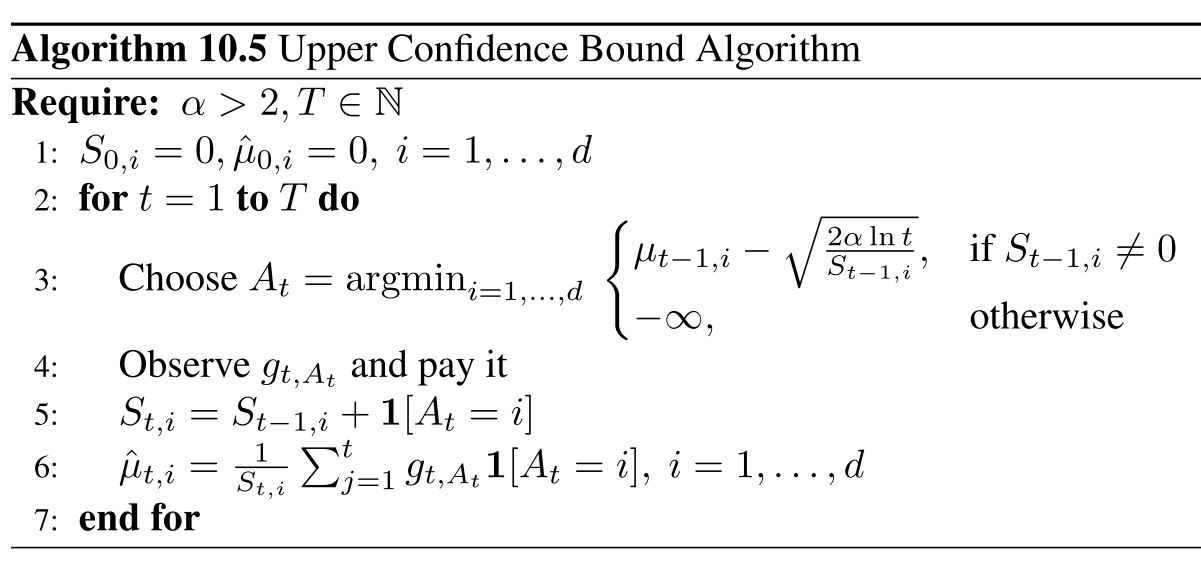
\includegraphics[width=0.75\textwidth]{./figures/UCB.png}
\end{figure}

\pause
UCB works keeping an estimate of the expected loss of each arm and also a confidence interval at a certain probability.


\end{frame}


\begin{frame}{UCB: Analysis}
\begin{theorem}
\label{thm:ucb}
Assume that the rewards of the arms are $1$-subgaussian and let $\alpha>2$. Then, UCB guarantees a regret of
\[
\mathrm{Regret}_T
\leq \frac{\alpha}{\alpha-2}\sum_{i=1}^d \Delta_i + \sum_{i: \Delta_i>0} \frac{8\alpha \ln T}{\Delta_i} ~.
\]
\end{theorem}
\end{frame}

\begin{frame}{UCB Regret Proof}
\begin{itemize}
\item Let $i=1$ be the optimal arm.

\item Note that $\mathrm{Regret}_T=\sum_{i=1}^d \Delta_i \mathbb{E}[S_{T,i}]$.
\item For arm non optimal arm $i$, we want to prove that $$\mathbb{E}[S_{T,i}]\leq \frac{8\alpha \ln T}{\Delta^2_i} + \frac{\alpha}{\alpha-2}$$.

\item The proof is based on the fact that once I have sampled an arm enough times, the probability to take a suboptimal
arm is small.

\item Let $t^\star$ the biggest time index such that $S_{t^\star-1,i} \leq \frac{8\alpha \ln T}{\Delta_i^2}$. 	For $t> t^\star$, we have 
\begin{equation}
\label{eq:thm_ucb_eq1}
S_{t-1,i} > \frac{8\alpha \ln T}{\Delta_i^2}~.
\end{equation}

\end{itemize}
\end{frame}

\begin{frame}{UCB Regret Proof}
\begin{itemize}

\item Consider $t> t^\star$ and such that $A_t = i \neq 1$, then we claim that at least one of the two following equations must be true:
\begin{align}
\hat{\mu}_{t-1,1} - \sqrt{\frac{2\alpha \ln t}{S_{t-1,1}}} &\geq \mu_1, \label{eq:ucb1}\\
\hat{\mu}_{t-1,i} + \sqrt{\frac{2\alpha \ln t}{S_{t-1,i}}} &< \mu_i~. \label{eq:ucb2}
%S_{i,t-1} &< \frac{2 \alpha \ln T}{ \Delta_i^2}~. \label{eq:ucb3}
\end{align}

\end{itemize}
\end{frame}


\begin{frame}{UCB Regret Proof}
Let's prove the claim: \emph{if both the inequalities above are false}, $t> t^\star$, and $A_t = i$, we have
\begin{align*}
\hat{\mu}_{t-1,1} - \sqrt{\frac{2\alpha \ln t}{S_{t-1,1}}} 
&< \mu_1 \qquad (\eqref{eq:ucb1} \text{ false}) \\
&= \mu_i - \Delta_i \\
&< \mu_i - 2\sqrt{\frac{2\alpha \ln T}{S_{t-1,i}}} \qquad (\text{for } \eqref{eq:thm_ucb_eq1})\\
&\leq \hat{\mu}_{t-1,i} - \sqrt{\frac{2 \alpha \ln t}{S_{t-1,i}}} \qquad (\eqref{eq:ucb2} \text{ false}),
\end{align*}
that, by the selection strategy of the algorithm, would imply $A_t \neq i$.

\end{frame}

\begin{frame}{UCB Regret Proof}
Note that $S_{t^\star,i} \leq \frac{8\alpha \ln T}{\Delta_i^2}+1$. Hence, we have
\begin{align*}
\mathbb{E}\left[ S_{T,i}\right]
&= \mathbb{E}[S_{t^\star,i}] + \sum_{t=t^\star+1}^T \mathbb{E}[\boldsymbol{1}[A_t=i, \eqref{eq:ucb1} \text{ or } \eqref{eq:ucb2} \text{ true}]] \\
&\leq \frac{8\alpha \ln T}{\Delta_i^2} + 1 + \sum_{t=t^\star+1}^T \mathbb{E}[\boldsymbol{1}[\eqref{eq:ucb1} \text{ or } \eqref{eq:ucb2} \text{ true}]] \\
&\leq  \frac{8\alpha \ln T}{\Delta_i^2} + 1 + \sum_{t=t^\star+1}^T \left(\Pr[\eqref{eq:ucb1} \text{ true}] + \Pr[\eqref{eq:ucb2} \text{ true}]\right)~.
\end{align*}

\end{frame}


\begin{frame}{UCB Regret Proof}
Now, we upper bound the probabilities in the sum. First, note that, given that the losses on the arms are i.i.d., we have
\begin{align*}
\left\{\hat{\mu}_{t-1,1} - \sqrt{\frac{2\alpha \ln t}{S_{t-1,1}}} \geq \mu_1 \right\}
&\subset \left\{\max_{s=1, \dots, t-1} \ \frac{1}{s}\sum_{j=1}^s g_{j,1} - \sqrt{\frac{2\alpha \ln t}{s}} \geq \mu_1\right\}\\
&= \bigcup_{s=1}^{t-1} \left\{\frac{1}{s}\sum_{j=1}^s g_{j,1} - \sqrt{\frac{2\alpha \ln t}{s}} \geq \mu_1\right\}
\end{align*}
\end{frame}


\begin{frame}
Hence, we have
\begin{align*}
\Pr[\eqref{eq:ucb1} \text{ true} ]
&\leq \sum_{s=1}^{t-1} \Pr\left[\frac{1}{s}\sum_{j=1}^s g_{j,1} - \sqrt{\frac{2\alpha \ln t}{s}} \geq \mu_1\right] \qquad \text{(union bound)}\\
&\leq \sum_{s=1}^{t-1} t^{-\alpha} 
= (t-1) t^{-\alpha}~.
\end{align*}
\end{frame}


\begin{frame}
Given that the same bound holds for $\Pr[\eqref{eq:ucb2} \text{ true}]$, we have
\begin{align*}
\mathbb{E}\left[ S_{T,i}\right] 
&\leq \frac{8\alpha \ln T}{\Delta_i^2} + 1 + \sum_{t=1}^{\infty} 2 (t-1) t^{-\alpha} \\
&\leq \frac{8\alpha \ln T}{\Delta_i^2} + 1 + \sum_{t=2}^{\infty} 2 t^{1-\alpha} \\
&\leq \frac{8\alpha \ln T}{\Delta_i^2} + 1 + 2\int_{1}^{\infty} x^{1-\alpha}\\
&=\frac{8\alpha \ln T}{\Delta_i^2} + \frac{\alpha}{\alpha-2}~.
\end{align*}
Using the decomposition of the regret we proved last time, $$\mathrm{Regret}_T=\sum_{i=1}^d \Delta_i \mathbb{E}[S_{T,i}],$$ we have the stated bound.
\end{frame}

\section{New Trends}

\frame{\sectionpage}

\subsection{Bandits}
\frame{\subsectionpage}

\begin{frame}{New Trends}
\framesubtitle{Exploration}
\begin{itemize}
\item 
Now suppose this problem:
\begin{enumerate}
\item 
Strategy chooses $a_t \in \mathcal{A} \subset \R^d$.
\item
Adversary chooses \textbf{linear} loss $l_t \in \mathcal{L} \subseteq [-1, 1]^ \mathcal{A}$
\item
Strategy sees loss  $l_t(a_t)= l_t^T a_t$

\end{enumerate}

We aim to minimize pseudo-regret:

\begin{equation}
{R_n}= \mathbb{E} \sum_{t=1}^T l_t(a_t) - \underset{a \in \mathcal{A}}{\mathrm{\min}} \sum_{t=1}^T l_t(a)
\end{equation}

\pause

problem falls to how to choose $a_t$'s. And how to estimate $l_t^T a$

\end{itemize}
\end{frame}


\begin{frame}{New Trends}
\framesubtitle{Exploration}
\begin{figure}[h!]
\centering
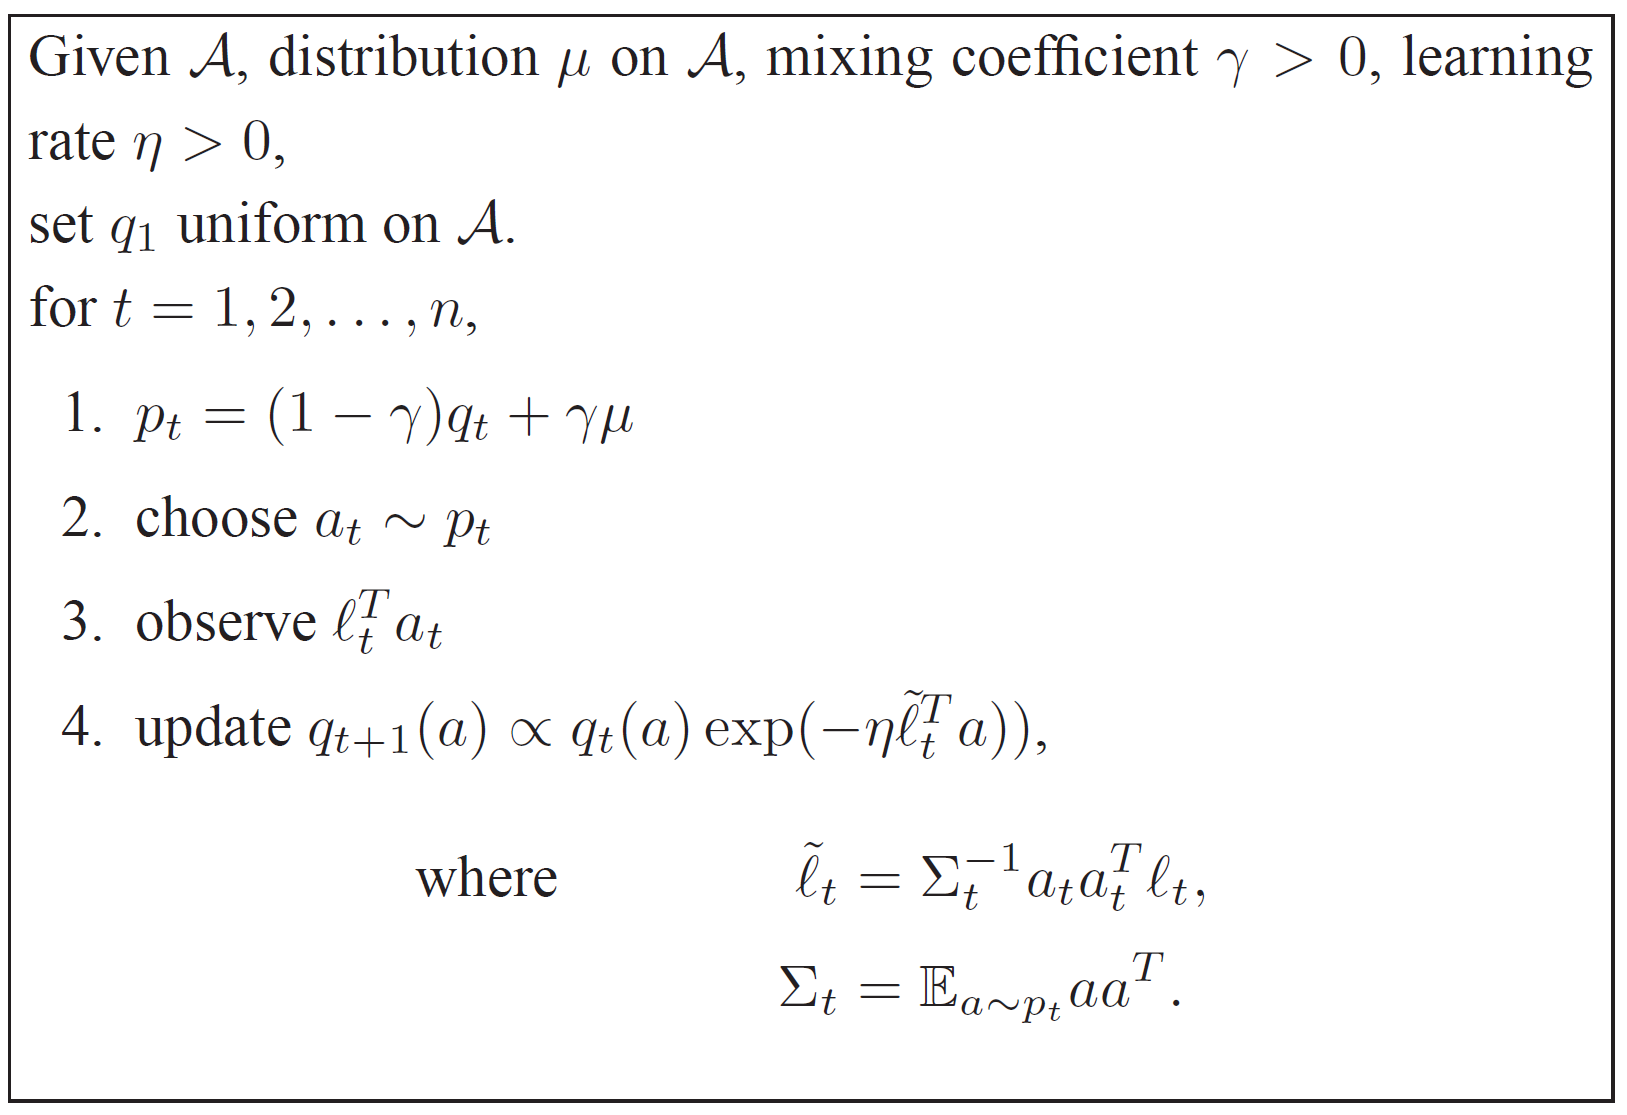
\includegraphics[width=0.8\textwidth]{./figures/Exploration.png}
\end{figure}    
\end{frame}


\begin{frame}{New trends}
\framesubtitle{Exploration}
\begin{itemize}
\item Strategy observes $a_t^T l_t$ and $a_t$, so it can compute:
$$ \tilde{l_t}= \Sigma_t^{-1} a_t (a_t^T l_t)$$

\item
$ \tilde{l_t}$ is unbiased:
$$ \mathbb{E}[\tilde{l_t} | \mathcal{F}_{t-1}]= (\mathbb{E}_{a \sim p_t} a a^T)^{-1} (\mathbb{E}_{a \sim p_t} a a^T) l_t= l_t.$$

\pause

\item
Therefore:
$$\mathbb{E}[l_t^T a]= E[\tilde{l_t}^T a] \ \ \forall a$$

\pause

\item
and:
$$\mathbb{E}[l_t^T a_t]= \E [\sum_{a \in \Ayp} p_t(a) \E[\tilde{l_t} |\mathcal{F}_{t-1}]^T a]
= \E[\sum_{a \in \Ayp} p_t(a) \tilde{l_t}^T a]$$

\end{itemize}
\end{frame}

\begin{frame}{New Trends}
\framesubtitle{Exploration}

\begin{itemize}
\item 
So we can write the strategy’s expected cumulative loss as:
$$ \E \sum_{t=1}^n l_t^T a_t= \E \sum_{t=1}^n \sum_{a \in \Ayp} p_t(a) \tilde{l_t}^T a.$$


\pause
\item
Which can be written as:
\begin{align*}
\sum_{t=1}^n \sum_{a \in \Ayp} p_t(a) \tilde{l_t}^T a &= \sum_{t=1}^n \sum_{a \in \Ayp} ((1-\gamma) q_t(a)+ \gamma \mu(a)) \tilde{l_t}^T a\\
&=  (1-\gamma)(\sum_{t=1}^n \sum_{a \in \Ayp} q_t(a) \tilde{l_t}^T a) + \gamma  (\sum_{t=1}^n \sum_{a \in \Ayp} \mu(a) \tilde{l_t}^T a)
\end{align*}


\end{itemize}

\end{frame}


\begin{frame}{New Trends}
\framesubtitle{Exploration}

\begin{itemize}
\item
Note that the ditrbution changes as well:

\begin{align*}
\E \sum_{t=1}^n (l(\tilde{a_t}, z_t)- l({a}, z_t)) &= \E \sum_{t=1}^n (l(\tilde{a_t}, z_t)- l({a_t}, z_t) + l({a_t}, z_t)- l({a}, z_t))\\
& \leq G \E \sum_{t=1}^n \|a_t-\tilde{a_t} \| + \E  \sum_{t=1}^n \nabla l(a_t, z_t)^T (a_t-a)\\
&= G \E \sum_{t=1}^n \|a_t-\tilde{a_t} \| + \E  \sum_{t=1}^n \tilde{l_t}^T (a_t-a)
\end{align*}

\item
In our case, if we assume $\| l_t \| \leq 1$:

$$\E \sum_{t=1}^n (l(\tilde{a_t}, z_t)- l({a}, z_t)) \leq 2 \gamma n + \E  \sum_{t=1}^n \tilde{l_t}^T (a_t-a)$$

\end{itemize}

\end{frame}

\begin{frame}{New Trends}
\framesubtitle{Exploration}

\begin{itemize}

\item 
Recall this theorem:
\begin{thm}
Assume that the normalized EG algorithm is run on a sequence of linear loss functions such that for all $t, i$ we have $\eta z_t[i] \geq -1$.
Then:

$$
\sum_{t=1}^T  \langle w_t-\uu , z_t \rangle \leq \frac{\log(d)}{\eta}  + \eta \sum_{t=1}^T \sum_i w_t[i] z_t[i]^2$$
\end{thm}

\pause

\item
\begin{align*}
\tilde{R}_n &\leq 2 \gamma n + (1- \gamma)(\frac{\log(N)}{\eta}  + \eta \E \sum_{t=1}^T \sum_{a \in \mathcal{A}}  q_t(a) (\tilde{l_t}^T a)^2)\\
& \leq 2 \gamma n + \frac{\log(N)}{\eta}  + \eta \sum_{t=1}^T \sum_{a \in \mathcal{A}}  p_t(a) (\tilde{l_t}^T a)^2
\end{align*}
\end{itemize}
\end{frame}

\begin{frame}{New Trends}
\framesubtitle{Exploration}
\begin{itemize}
\item 
\begin{align*}
\sum_{a \in \mathcal{A}}  p_t(a) \langle \tilde{l_t}, a \rangle ^2 &= \sum_{a \in \mathcal{A}}  p_t(a) \langle \tilde{l_t}, (a a^T) \tilde{l_t} \rangle\\
&= \langle \tilde{l_t}, \Sigma_t \tilde{l_t} \rangle\\
&=  \langle a_t, l_t \rangle ^2 \langle \Sigma_t^{-1} a_t, \Sigma_t \Sigma_t^{-1} a_t \rangle
\end{align*}
where in last equality, we've used: $\tilde{l_t}= \Sigma_t^{-1} a_t \langle a_t, l_t \rangle$

\pause

\item
if we assume $\|a \| \leq 1$, we will have:
$$ \leq \langle \Sigma_t^{-1} a_t,  a_t \rangle$$

\pause

\item
$$\E \langle \Sigma_t^{-1} a_t,  a_t \rangle= d!$$

\end{itemize}
\end{frame}

\begin{frame}{New Trends}
\framesubtitle{Exploration}
\begin{itemize}
\item We now turn to $\langle a, \tilde{l_t} \rangle$ (Why?)

\begin{align*}
\langle a, \tilde{l_t} \rangle &= \langle a_t, l_t \rangle \langle a_t, \Sigma_t^{-1}  a_t \rangle\\
&= \langle a_t, \Sigma_t^{-1}  a_t \rangle \\
& \leq \frac{1}{min_{1 \leq i \leq d} \lambda_i}
\end{align*}

\pause

\item
We must have:
$$\eta z_t[i] \geq -1$$
to guarantee normalized EG algorithm.

\end{itemize}
\end{frame}

\begin{frame}{New Trends}
\framesubtitle{Exploration}
\begin{thm}
Assume that $\mathcal{L} \subset [-1, 1]^\mathcal{A}$, if:

$$ \underset{a, b \in \mathcal{A}}{a^t \Sigma_t^{-1} b } \leq  \frac{c_d}{\gamma}$$

setting $\gamma= c_d \eta, \eta= \sqrt{\frac{\log(N)}{n(d+ c_d)}}$, wo will have:
\begin{equation}
\tilde{R_n} \leq 2 \sqrt{n(c_d+ d) \log(N)}
\end{equation}
\end{thm}

\pause

Getting back to exploration term, what should we set for $\mu(a)$ to guarantee above bound?
\end{frame}

\begin{frame}{New Trends}
\framesubtitle{Exploration}
\begin{figure}[h!]
\centering
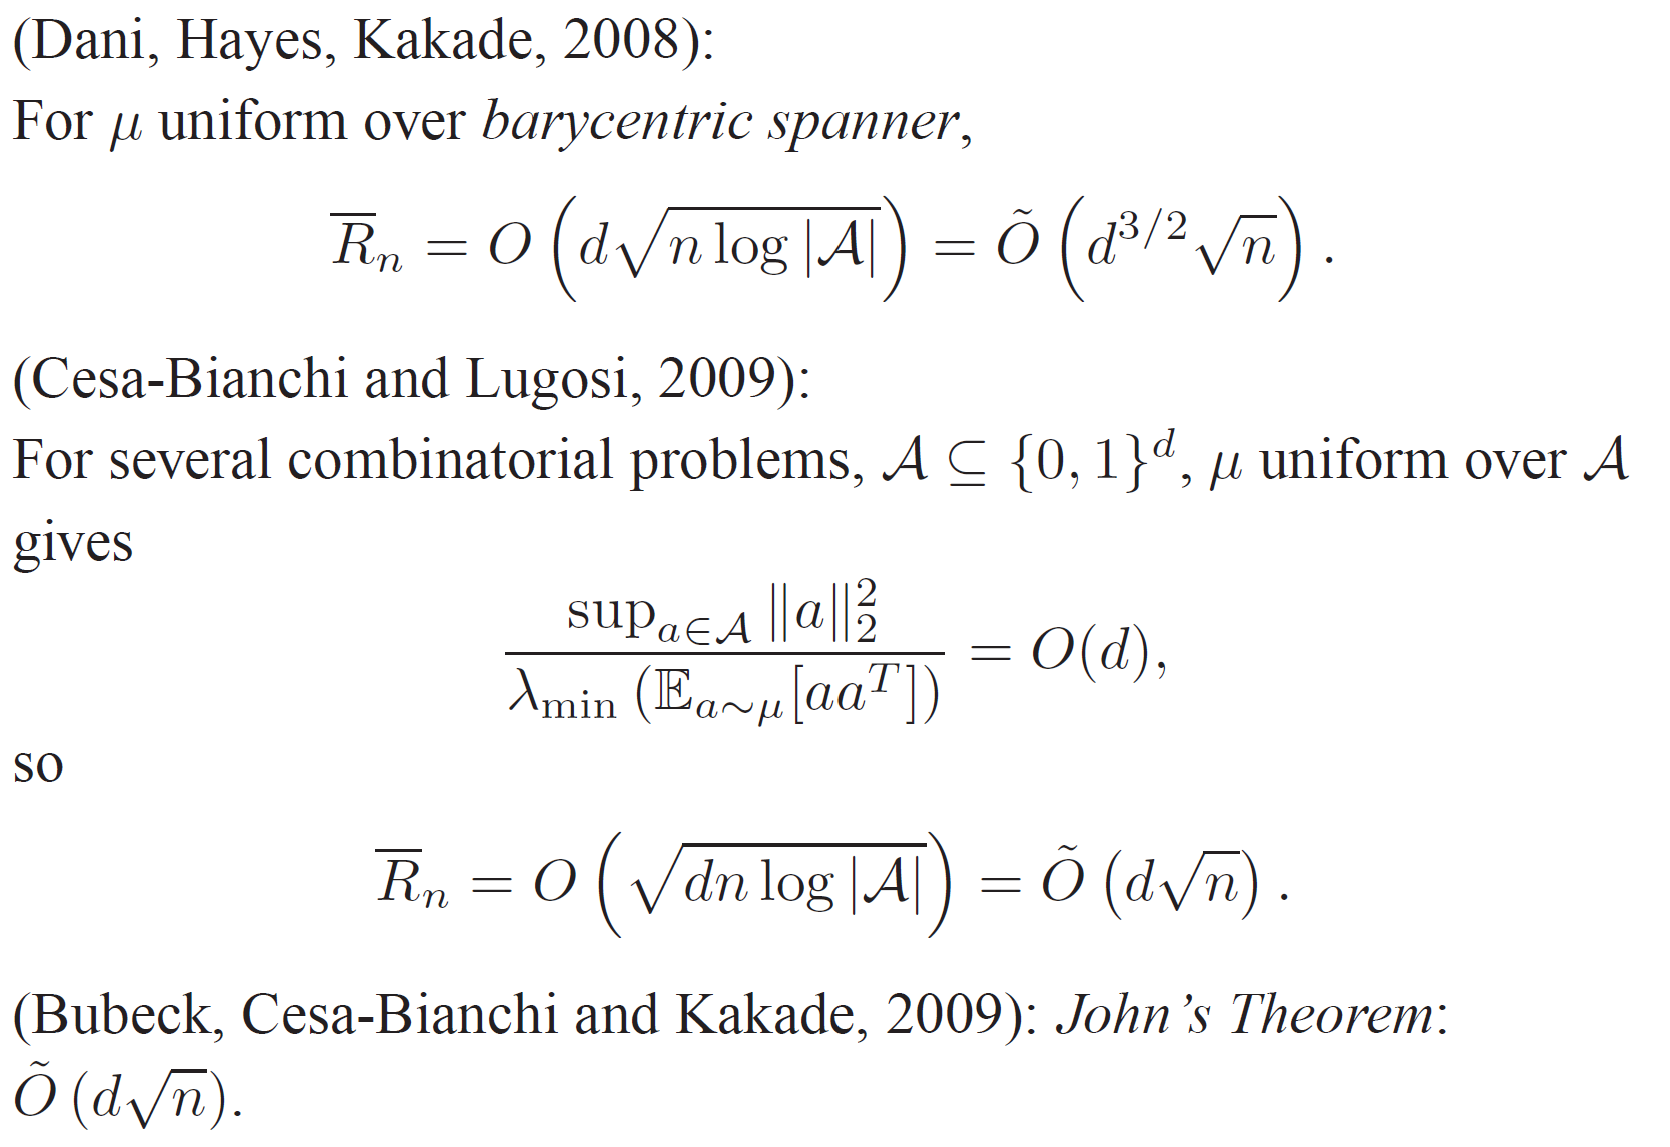
\includegraphics[width=0.8\textwidth]{./figures/different_exploration.png}
\end{figure}

\end{frame}


\begin{frame}{New Trends}
\framesubtitle{barycentric spanner}
\begin{itemize}
\item 
Suppose that $\Ayp \subset \R ^d$ spans $\R ^ d$, a barycentric spanner of $\mathcal{A}$ is a set ${b_1, \hdots , b_d}$ that spans $\R ^d$ and satisfies:

for all $a \in  \mathcal{A}$ there is an $\alpha \in [-1, 1]^d$ such that $a = B \alpha$, where $B= (b_1, \hdots, b_d)$.

it can be shown that:

\pause
Every compact $\Ayp$ has a barycentric spanner.

\pause
If linear functions can be efficiently optimized over A, then there is an efficient algorithm for finding an approximate barycentric spanner. That is: $|\alpha_i|< 1+ \delta$ then it needs $O(d^2 \log(d) / \delta)$
\end{itemize}
\end{frame}


\begin{frame}{New Trends}
\framesubtitle{barycentric spanner}
\begin{block}{Lemma}
If ${b_1, \hdots, b_d} \subset A$ maximizes $det(B)$, then it is a barycentric spanner.
\end{block}

\pause

\begin{proof}
For $a= B \alpha$:

\begin{align*}
|det(B)| &\geq |det(a, b_2, \hdots, b_d)| \\
&= |\sum_i \alpha_i det(b_i, b_2, \hdots, b_d)|\\
&= |\alpha_1| |det(B)|
\end{align*}

\end{proof}
\end{frame}


\begin{frame}{New Trends}
\framesubtitle{barycentric spanner}
\begin{figure}[h!]
\centering
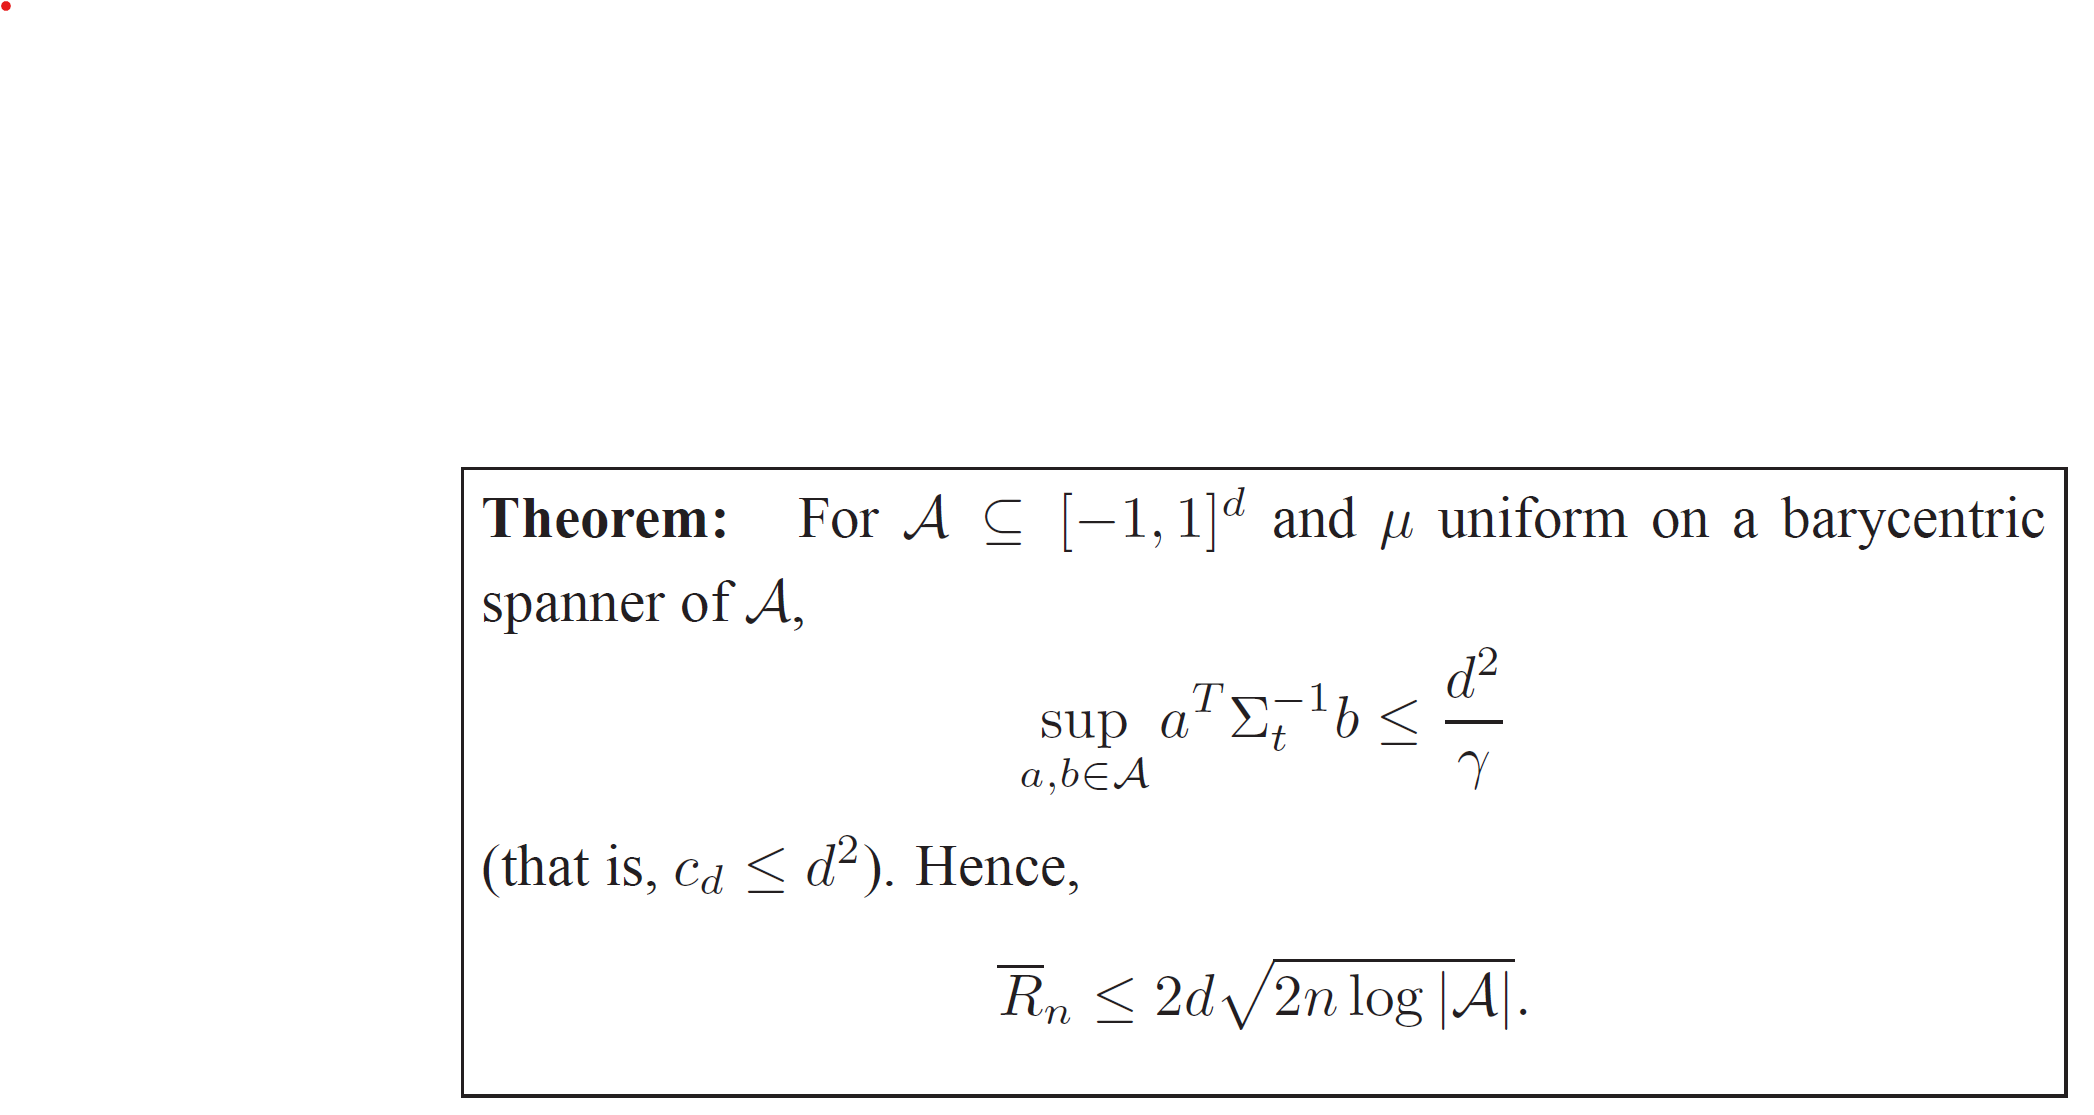
\includegraphics[width=0.8\textwidth]{./figures/Barry_proof.png}
\end{figure}
\end{frame}





\subsection{Parameter-Free Online Learning}
\frame{\subsectionpage}

\begin{frame}
\frametitle{New Trends}
\framesubtitle{Parameter-Free Online Learning}

\begin{itemize}
\item Using OGD with 1-Lipschitz losses and learning rate $\eta = \frac{\alpha}{T}$, we arrive at the following Regret bound:

\begin{equation}
\mathrm{Regret}_T(\uu) \leq \frac{||\uu||_2^2}{2\eta} + \frac{\eta T}{2} = \frac{1}{2} \sqrt{T} \Big(\frac{||\uu||_2^2}{\alpha} + \alpha\Big)
\end{equation}

\item To get the best bound, we need to set $\alpha = ||\uu||_2$.

\pause	
\item \textbf{Goal}: Design OCO algorithms that will enjoy the optimal regret and will not require any parameter.

\begin{itemize}
\item Doubling Trick --- Sub-optimal.
\item \textbf{Coin-Betting}
\end{itemize}

\end{itemize}
\end{frame}


\begin{frame}
\frametitle{New Trends}
\framesubtitle{Parameter-Free Online Learning: Coin Betting}
Imagine the following repeated game to maximize $\mathrm{Wealth_T}$:

\begin{itemize}
\item Set initial weight to $\epsilon$: $\mathrm{Wealth}_0 = \epsilon$.

\item In each round $t = 1, \dots, T$:
\begin{itemize}
\item You bet $x_t = \beta_t \mathrm{Wealth}_t$ where $|\beta_t| \leq 1$ on side on coin $\mathrm{sign}(\beta_t)$. 

\item The adversary reveals coin $c_t \in \{-1, 1\}$.

\item $\mathrm{Wealth}_t = \mathrm{Wealth}_{t-1} + c_tx_t = (1+\beta_tc_t) \mathrm{Wealth}_{t-1}$
\end{itemize}

\item This is a special instance of OCO, and we can have algorithms guaranteeing high $\mathrm{Wealth_T}$.
\begin{itemize}
\item \textbf{KT Betting}: $\beta_t = \frac{\sum_{i= 1}^{t-1}c_i}{t}$.

\item Guarantee: 

$$\ln(\mathrm{Wealth}_T) \geq \sum_{t = 1}^{T} \frac{\big(\sum_{i = 1}^{T} c_t\big)^2}{4T} - \frac{1}{2}\log(T)$$
\end{itemize}
\end{itemize}
\end{frame}


\begin{frame}
\frametitle{New Trends}
\framesubtitle{Parameter-Free Online Learning: Coin Betting}

\begin{block}{Theorem}
Let $\phi$ be a proper closed convex function and let $\phi^*$ be its Fenchel conjugate. If an algorithm that generates $\x_1, \x_2, \dots, \x_n \in\mathbb{R}^d$ can guarantee

$$\forall \mathbf{g_1}, \mathbf{g_2}, \dots, \mathbf{g_T} \in \mathbb{R}^d: \;\; \epsilon - \sum_{t = 1}^{T}\langle\x_t, \mathbf{g}_t\rangle \geq \epsilon - \sum_{t = 1}^{T} \phi\big(-\sum_{t = 1}^{T} \mathbf{g}_t\big),$$
Then it guarantees 
$$\forall \uu \in \mathbb{R}^d, \;\; \sum_{t = 1}^{T}\langle \mathbf{g}_t, \x_t - \uu \rangle \leq \phi^*(\uu) + \epsilon$$
\end{block}
\end{frame}


\begin{frame}
\frametitle{New Trends}
\framesubtitle{Parameter-Free Online Learning: Coin Betting}
\begin{itemize}

\item Assumption: $\forall \mathbf{g_1}, \mathbf{g_2}, \dots, \mathbf{g_T} \in \mathbb{R}^d: \;\; \epsilon - \sum_{t = 1}^{T}\langle\x_t, \mathbf{g}_t\rangle \geq \epsilon - \sum_{t = 1}^{T} \phi\big(-\sum_{t = 1}^{T} \mathbf{g}_t\big)$

\vspace{0.5cm}
\pause
\item  The Regret can be bounded as follows:

\begin{align*}
\sum_{t = 1}^{T}\langle \mathbf{g}_t, \x_t - \uu \rangle &\leq - \sum_{t = 1}^{T}\langle \mathbf{g}_t, \uu\rangle - \phi\big(-\sum_{t = 1}^{T} \mathbf{g}_t\big) + \epsilon\\
&\leq \sup_{\theta \in \mathbb{R}^d} \langle \theta, \uu \rangle - \phi(\theta) + \epsilon = \phi^*(\uu) + \epsilon
\end{align*}

\end{itemize}
\end{frame}

\begin{frame}
\frametitle{New Trends}
\framesubtitle{Parameter-Free Online Learning: Coin Betting}

\begin{itemize}


\item The regret guarantee of KT used a 1d OLO algorithm is upper bounded by

\small{\[
\mathrm{Regret}_T(u)
=\sum_{t=1}^T \ell_t(x_t) - \sum_{t=1}^T \ell_t(u)
\leq |u| \sqrt{4 T \ln \left(\frac{\sqrt{2} |u| K T }{\epsilon}+1\right)} + \epsilon, \ \forall u \in \R,
\]}

\item To better appreciate this regret, compare this bound to the one of OMD with learning rate $\eta=\frac{\alpha}{\sqrt{T}}$:
\[
\mathrm{Regret}_T(u)
=\sum_{t=1}^T \ell_t(x_t) -\sum_{t=1}^T \ell_t(u)
\leq \frac{1}{2}\left(\frac{u^2}{\alpha}+\alpha\right)\sqrt{T}, \ \forall u \in \R~.
\]

\pause

\item How to generalize to the general setting? Magnitude and Direction Decomposition

\end{itemize}
\end{frame}


\begin{frame}
\frametitle{New Trends}
\framesubtitle{Parameter-free in Any Norm}

How should we convert the 1D algorithm to the general case?

\pause
\begin{figure}
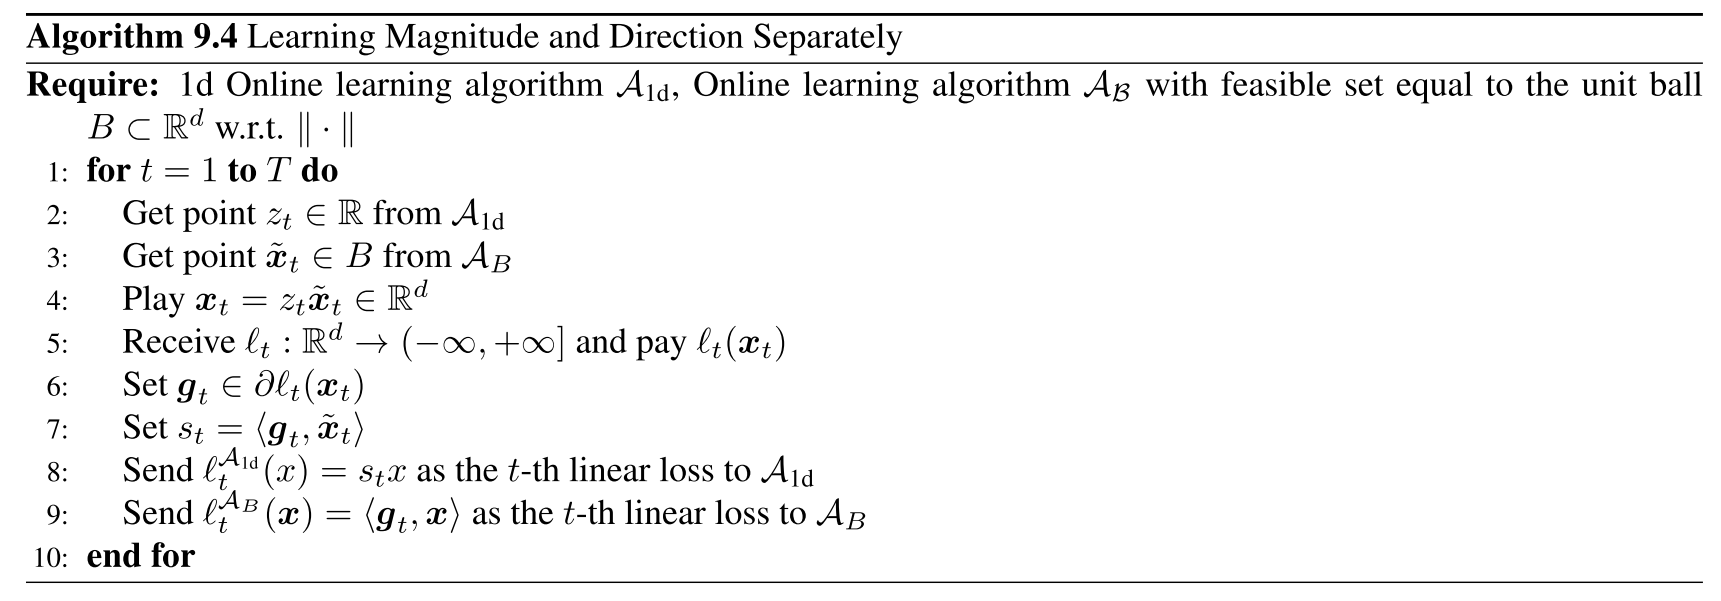
\includegraphics[width=\linewidth]{./figures/anyNorm.png}
\end{figure}
\end{frame}

\begin{frame}
\frametitle{New Trends}
\framesubtitle{Parameter-free in Any Norm}
\begin{theorem}
\begin{small}

\begin{align*}
\mathrm{Regret}_T(\uu) &\leq \sum_{t=1}^T \langle \mathbf{g}_t, \x_t -\uu\rangle
= \mathrm{Regret}^{\mathcal{A}_{\text{1d}}}_T(\|\uu\|) + \|\uu\| \mathrm{Regret}^{\mathcal{A}_{B}}_T\left(\frac{\uu}{\|\uu\|}\right)~.
\end{align*}
\end{small}
Further, the subgradients $s_t$ sent to $\mathcal{A}_{\text{1d}}$ satisfy $|s_t|\le \|\mathbf{g}_t\|_\star$.
\end{theorem}
\end{frame}

\begin{frame}
\begin{align*}
\mathrm{Regret}_T(\uu)
&\leq \sum_{t=1}^T \langle \mathbf{g}_t, \x_t - \uu\rangle
= \sum_{t=1}^T \langle \mathbf{g}_t, z_t \tilde{\x}_t\rangle - \langle \mathbf{g}_t, \uu\rangle\\
&= \underbrace{\sum_{t=1}^T \left(\langle \mathbf{g}_t, \tilde{\x}_t \rangle z_t - \langle \mathbf{g}_t, \tilde{\x}_t\rangle \|\uu\|\right)}_{\text{linear regret of }\mathcal{A}_{\text{1d}}\text{ at } \|\uu\| \in \R} + \sum_{t=1}^T \left(\langle \mathbf{g}_t, \tilde{\x}_t \rangle \|\uu\|  - \langle \mathbf{g}_t, \uu \rangle \right)\\
&= \mathrm{Regret}^{\mathcal{A}_{\text{1d}}}_T(\|\uu\|) + \sum_{t=1}^T \left(\langle \mathbf{g}_t, \tilde{\x}_t\rangle \|\uu\|  - \langle \mathbf{g}_t, \uu\rangle \right)\\
&= \mathrm{Regret}^{\mathcal{A}_{\text{1d}}}_T(\|\uu\|) +\|\uu\| \sum_{t=1}^T \left(\langle \mathbf{g}_t, \tilde{\x}_t\rangle - \left\langle \mathbf{g}_t, \frac{\uu}{\|\uu\|}\right\rangle \right)\\
&= \mathrm{Regret}^{\mathcal{A}_{\text{1d}}}_T(\|\uu\|) + \|\uu\| \mathrm{Regret}^{\mathcal{A}_{B}}_T\left(\frac{\uu}{\|\uu\|}\right)~. \qedhere
\end{align*}
\end{frame}

\begin{frame}
\frametitle{New Trends}
\framesubtitle{Related Papers}
\begin{small}
\begin{itemize}

{\small
\item Orabona and P\'{a}l. \textit{Open Problem: Parameter-Free and Scale Free Online Learning}, COLT Open Problems, 2016.

\item Orabona and P\'{a}l.  \textit{Coin Betting and Parameter-free Online Learning}, NIPS 2016.

\item Kwang-Sung and Orabona.
\textit{Parameter-Free Online Convex Optimization with Sub-Exponential Noise}, COLT 2019.


\item Chen, Langford, and Orabona. \textit{Better Paratemer-free Stochastic Optimization with ODE Updates for Coin Betting}, Arxiv 2020.


\item Cutkosky, and Orabona; \textit{Black-Box Reductions for Parameter-Free Online Learning in Banach Spaces}, COLT 2018.

}
\end{itemize}
\end{small}

\end{frame}

\subsection{Combining Online Learning Guarantees}
\frame{\subsectionpage}

\begin{frame}
\frametitle{New Trends}
\framesubtitle{Combining Online Learning Guarantees}

\begin{theorem}
{\scriptsize Let $\mathcal{A}_1$ and $\mathcal{A}_2$ two OLO algorithms that produces the predictions $\x_{t,1}$ and $\x_{t,2}$ respectively.
Then, predicting with $\x_t=\x_{t,1}+\x_{t,2}$, guarantees:
\[
\sum_{t=1}^T \langle \mathbf{g}_t, \x_t\rangle - \sum_{t=1}^T \langle \mathbf{g}_t, \uu\rangle
= \min_{\uu=\uu_1+\uu_2} \ \mathrm{Regret}^{\mathcal{A}_1}_T(\uu_1) + \mathrm{Regret}^{\mathcal{A}_2}_T(\uu_2)~.
\]}
\end{theorem}
\begin{small}
\begin{proof}
Set $\uu_1+\uu_2=\uu$. Then,
{\scriptsize
\[
\sum_{t=1}^T \langle \mathbf{g}_t, \x_t\rangle - \sum_{t=1}^T \langle \mathbf{g}_t, \uu\rangle
=\sum_{t=1}^T \langle \mathbf{g}_t, \x_{t,1}\rangle - \sum_{t=1}^T \langle \mathbf{g}_t, \uu_1\rangle 
+\sum_{t=1}^T \langle \mathbf{g}_t, \x_{t,2}\rangle - \sum_{t=1}^T \langle \mathbf{g}_t, \uu_2\rangle~. \qedhere
\]}
\end{proof}
\vspace{-0.3cm}
\begin{itemize}
\item Cutkosky; \textit{Combining Online Learning Guarantees}, COLT 2020.
\end{itemize}

\end{small}
\end{frame}

\subsection{Predictable Sequences (a.k.a. Hints)}
\frame{\subsectionpage}

\begin{frame}
\frametitle{New Trends}
\framesubtitle{Predictable Sequences (a.k.a. Hints)}

\begin{itemize}
\item Regret guarantees can be loose if the sequence being encountered is not “worst-case”.

\item We have a hint or predict of what the adversary is going to play next.

\pause
\item \textbf{Online Learning with Predictable Gradient Sequences}:
\vspace{-0.2cm}
\begin{align*}
&	f_t \in \argmin_{f\in\mathcal{F}} \eta \langle f, M_t \rangle + D_R(f, g_{t-1})\\
&   g_t \in \argmin_{g\in\mathcal{F}} \eta \langle g, \nabla l_t \rangle + D_R(g, g_{t-1})
\end{align*}

\item $\mathrm{Regret}_T(\uu) \leq \eta^{-1}R^2 + \frac{\eta}{2} \sum_{t = 1}^{T}||\nabla l_t - M_t||_*^2$
\end{itemize}

\end{frame}


\begin{frame}
\frametitle{New Trends}
\framesubtitle{Predictable Sequences (a.k.a. Hints)}
\begin{columns}
\begin{column}{0.5\textwidth}
\begin{itemize}
\item At time $t$, adversary can play in $B_t$.
\item Regret bounds available for $B_t = \{ \w: \angle (\w, \mathbf{M}_t) \leq \alpha  \}$


\item What about a more general case?
\end{itemize}

\end{column}
\begin{column}{0.5\textwidth}  %%<--- here
\begin{figure}
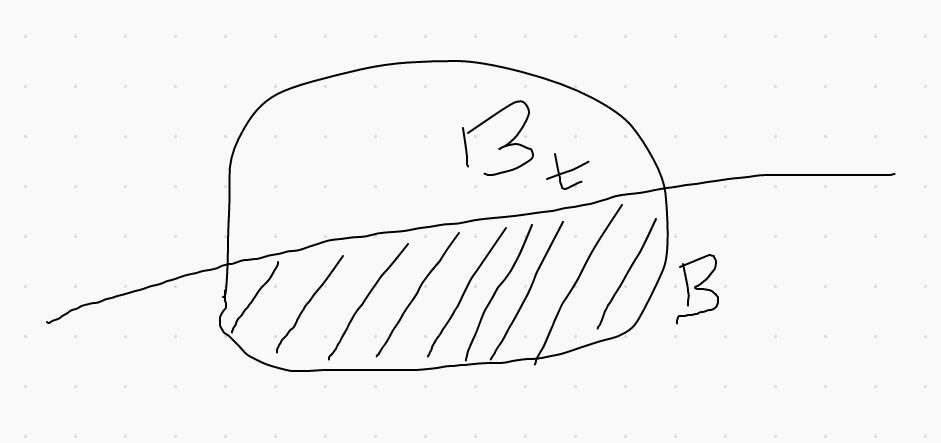
\includegraphics[scale=0.15]{./figures/hints.png}
\end{figure}
\end{column}
\end{columns}



\pause 


\begin{itemize}
\item \textbf{Some Papers}:	


\begin{itemize}
{\scriptsize
\item Rakhlin, Sridharan; \textit{Optimization, Learning and Games with Predictable Sequences}, NIPS 2013.

\item Rakhlin, Sridharan; \textit{Online Learning with Predictable Sequences}, COLT 2013.

\item Dekel, Flajolet, Haghtalab, Jaillet; \textit{Online Learning with a Hint}, NIPS 2017.

\item  Bhaskara, Cutkosky, Kumar and Purohit; \textit{Online Learning with Imperfect Hints}, ICML 2020. }
\end{itemize}

\end{itemize}

\end{frame}


\section{Bibliography}
\frame{\sectionpage}

\begin{frame}
\frametitle{Bibliography}
There are several good texts for a start:

\begin{enumerate}
{\small
\item Shai Shalev-Shwartz, \textit{Online Learning and Online
Convex Optimization}, Foundations and Trends in Machine Learning, 2011.

\item Francesco Orabona, \textit{A Modern Introduction to Online Learning},  ArXiv, 2020.

\item Tor Lattimore and Csaba Szepesv\'{a}ri, \textit{Bandit Algorithms},  Cambridge University Press, 2020.}
\end{enumerate}

\end{frame}

\end{document}